\newpage
\section{CHƯƠNG 3: Phân tích thiết kế hệ thống}

\subsection{Phân Tích Hệ Thống}

\subsubsection{Biểu đồ Usecase}


\textbf{Use Case Tổng quát} \\
\begin{figure}[H]
    \centering
    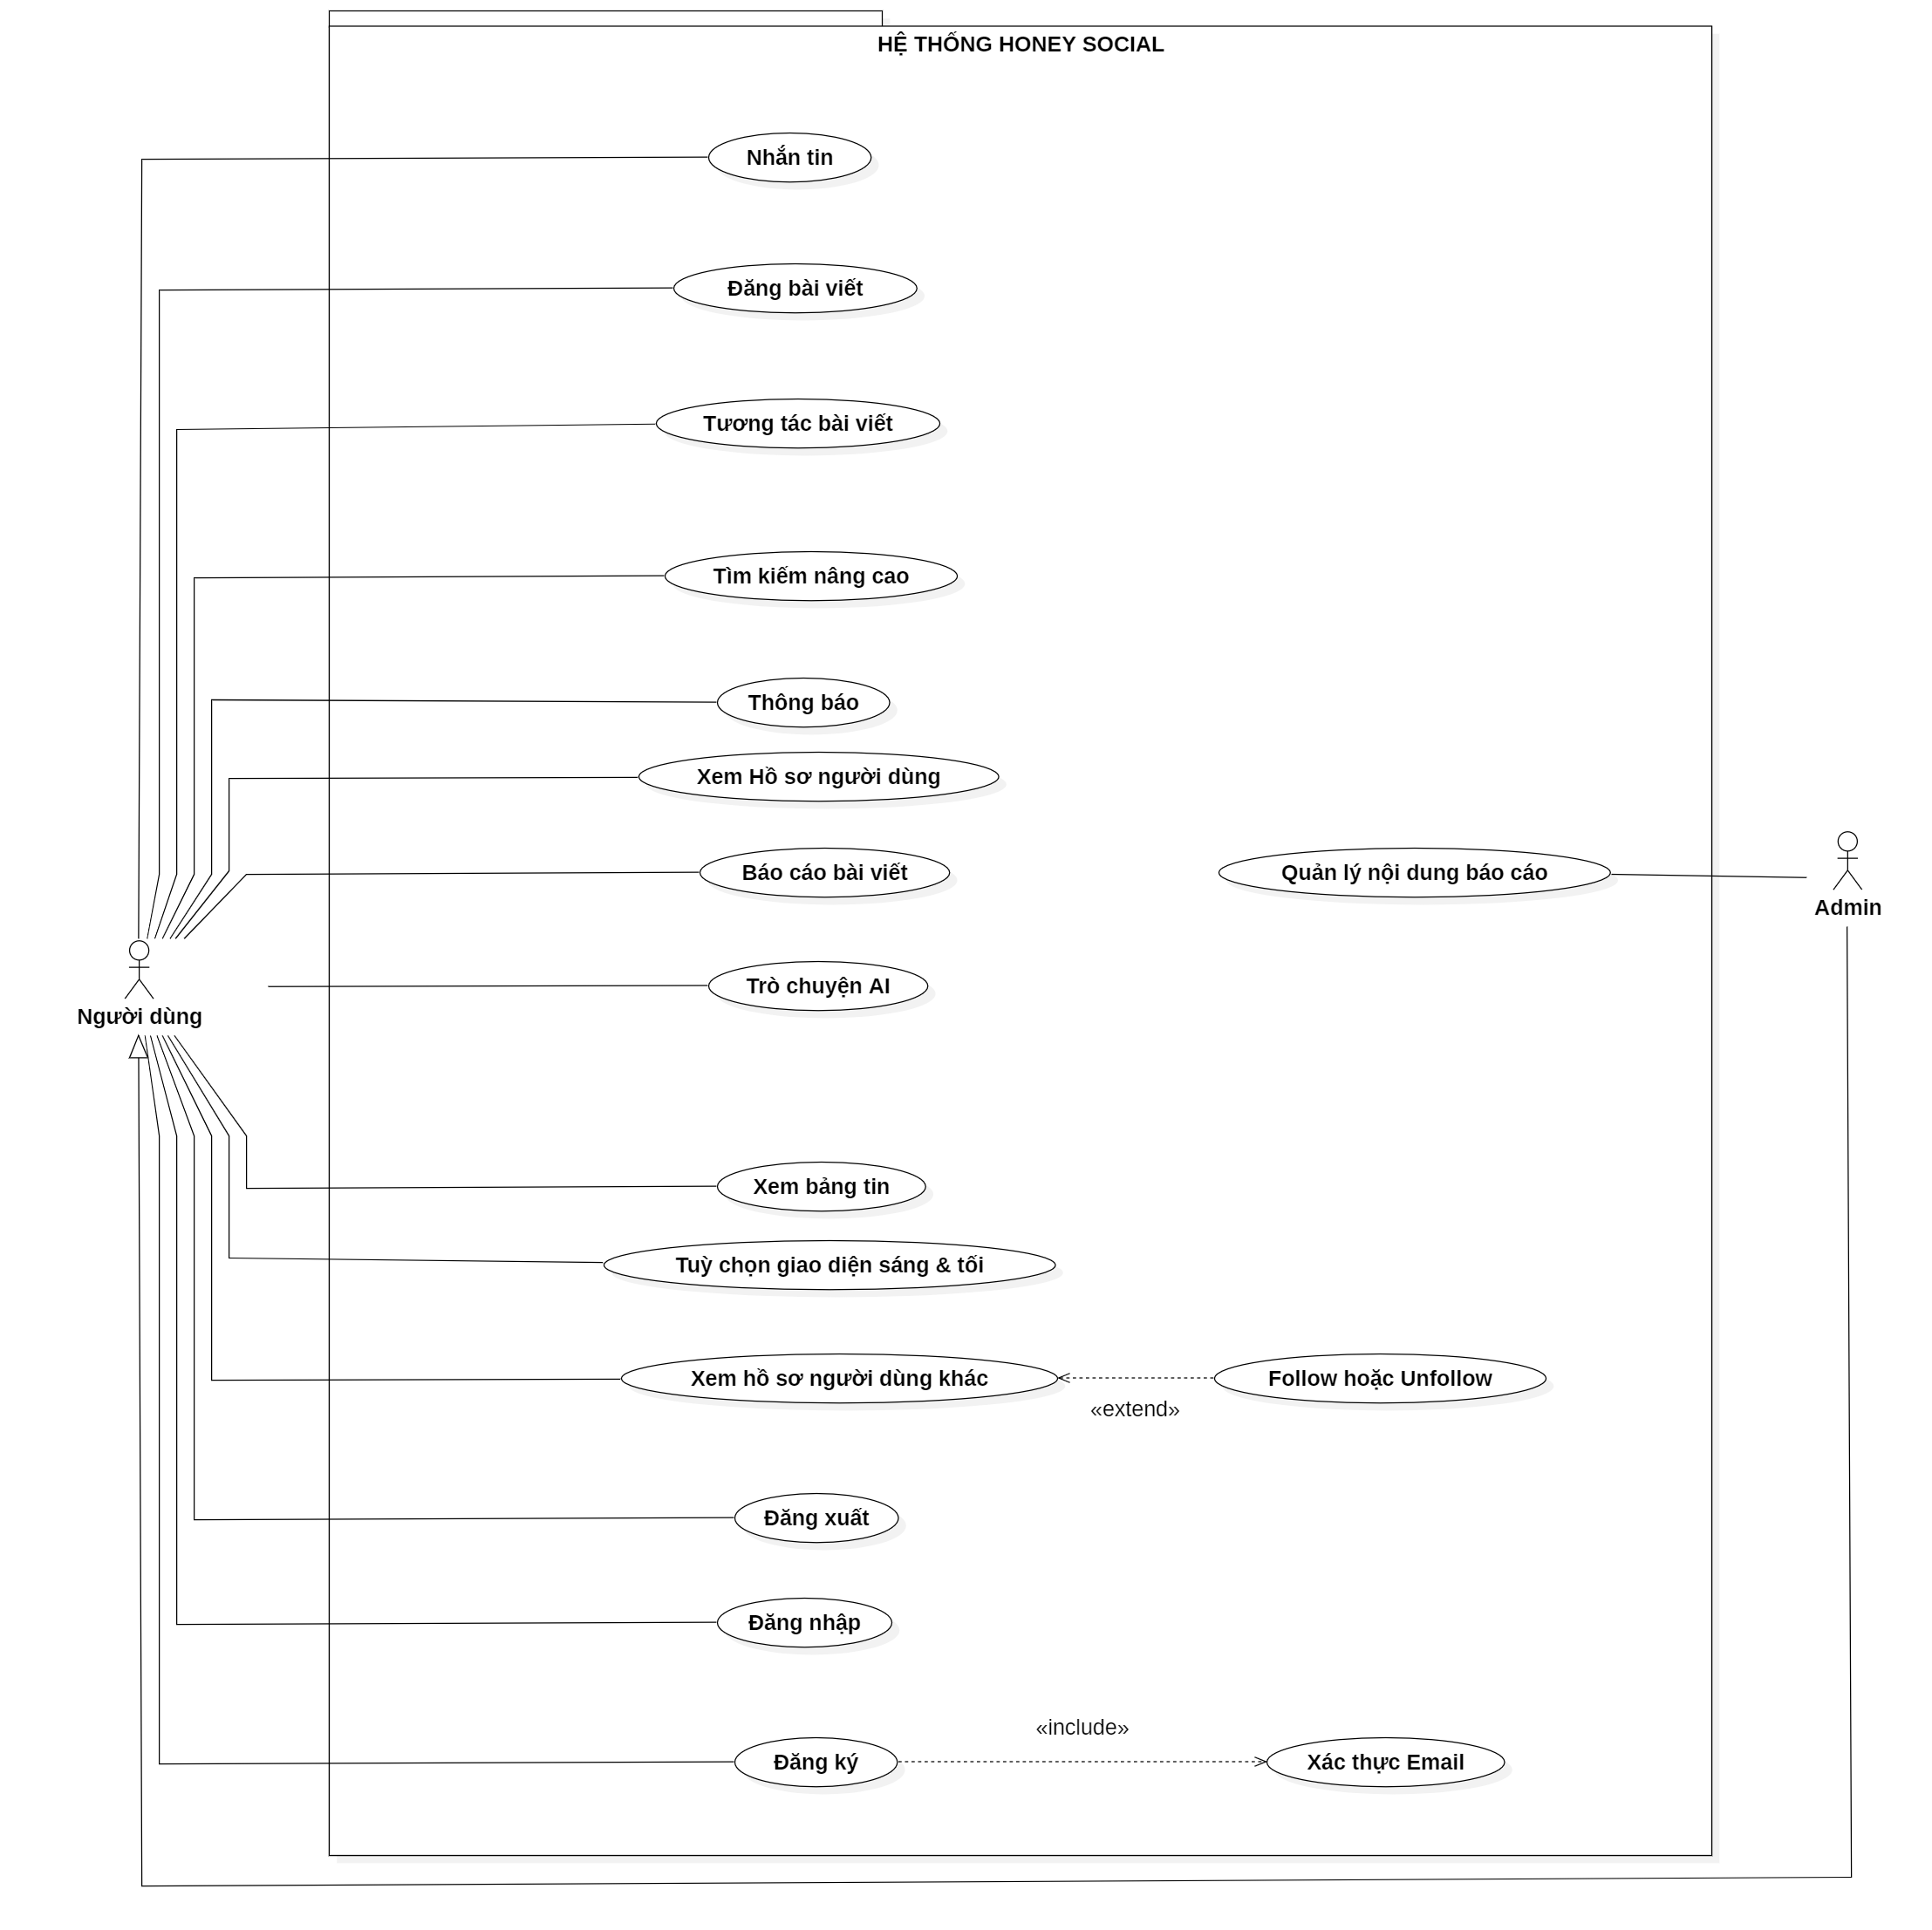
\includegraphics[width=1\textwidth]{image/MoHinh/1.png}
    \caption{Hình ảnh Use Case Tổng quát}
    \label{fig:use_case_tong_quat}
\end{figure}
Các chức năng được bao bởi hệ thống \textbf{HỆ THỐNG HONEY SOCIAL} và là những hành động mà người dùng có thể thực hiện như sau:

\begin{itemize}
    \item Nhắn tin
    \item Đăng bài viết
    \item Tương tác bài viết: Thích, bình luận, chia sẻ,...
    \item Tìm kiếm nâng cao
    \item Thông báo
    \item Xem hồ sơ người dùng
    \item Báo cáo bài viết
    \item Trò chuyện AI
    \item Xem bảng tin
    \item Tùy chọn giao diện sáng \& tối
    \item Đăng nhập
    \item Đăng xuất
\end{itemize}

\textbf{Đăng bài viết} \\
\begin{figure}[H]
    \centering
    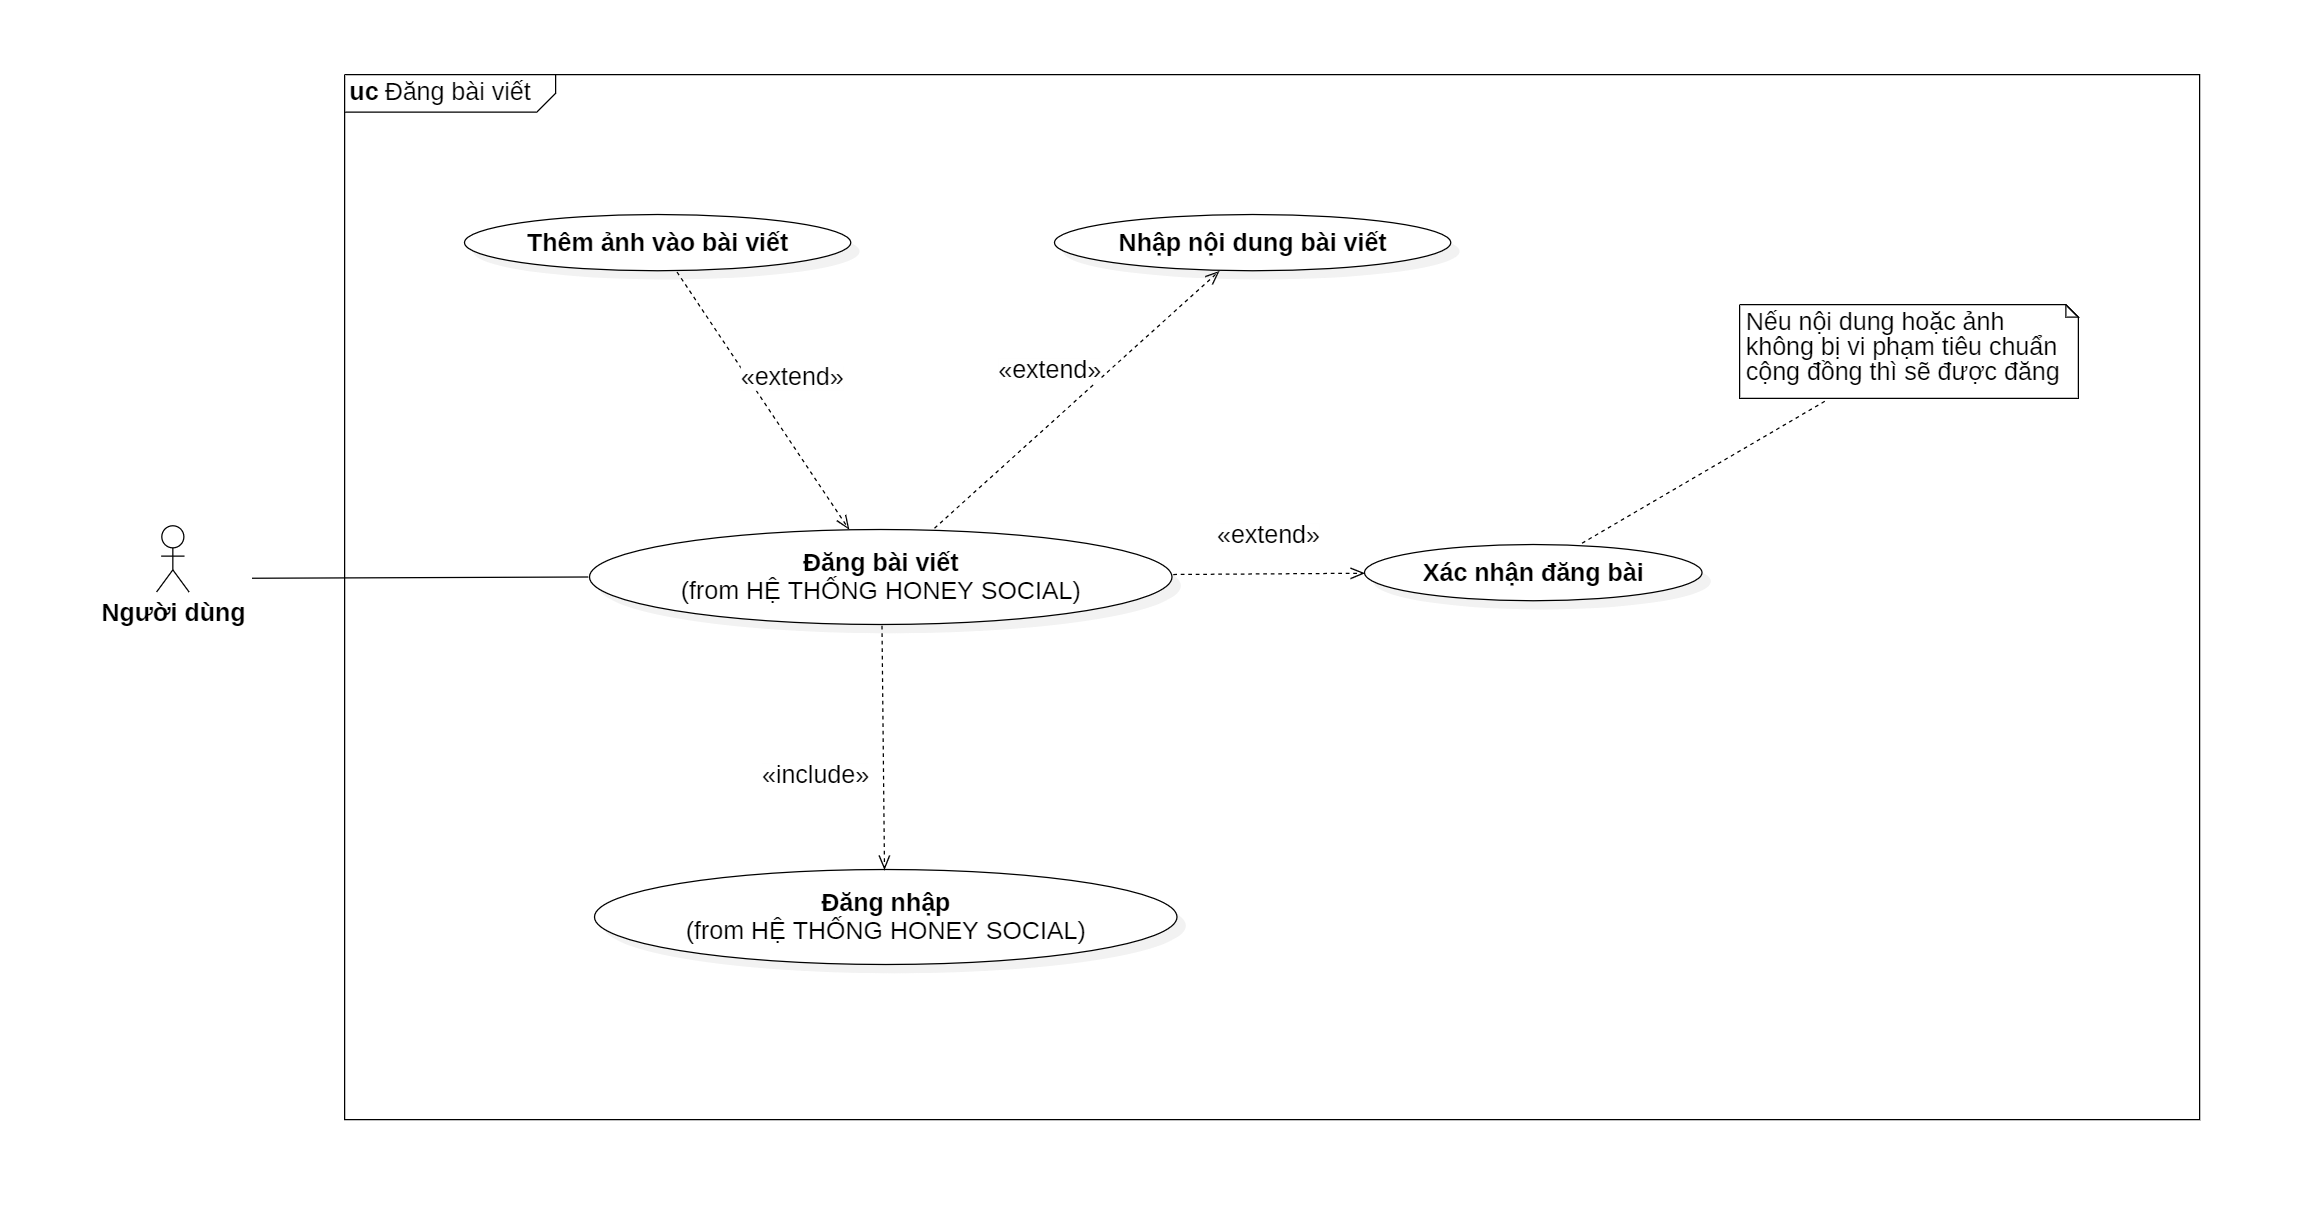
\includegraphics[width=1\textwidth]{image/MoHinh/2.png}
    \caption{Hình ảnh Đăng bài viết}
    \label{fig:dang_bai_viet_seq}
\end{figure}
Mô tả chi tiết quy trình đăng bài, bắt đầu từ việc người dùng nhập nội dung văn bản, tải lên ảnh hoặc video, chỉnh sửa trước khi đăng (bao gồm thêm hashtag hoặc thẻ người), trải qua kiểm duyệt tự động bằng AI, và cuối cùng là xác nhận để bài viết được công khai trên bảng tin.

\textbf{Tìm kiếm nâng cao} \\
\begin{figure}[H]
    \centering
    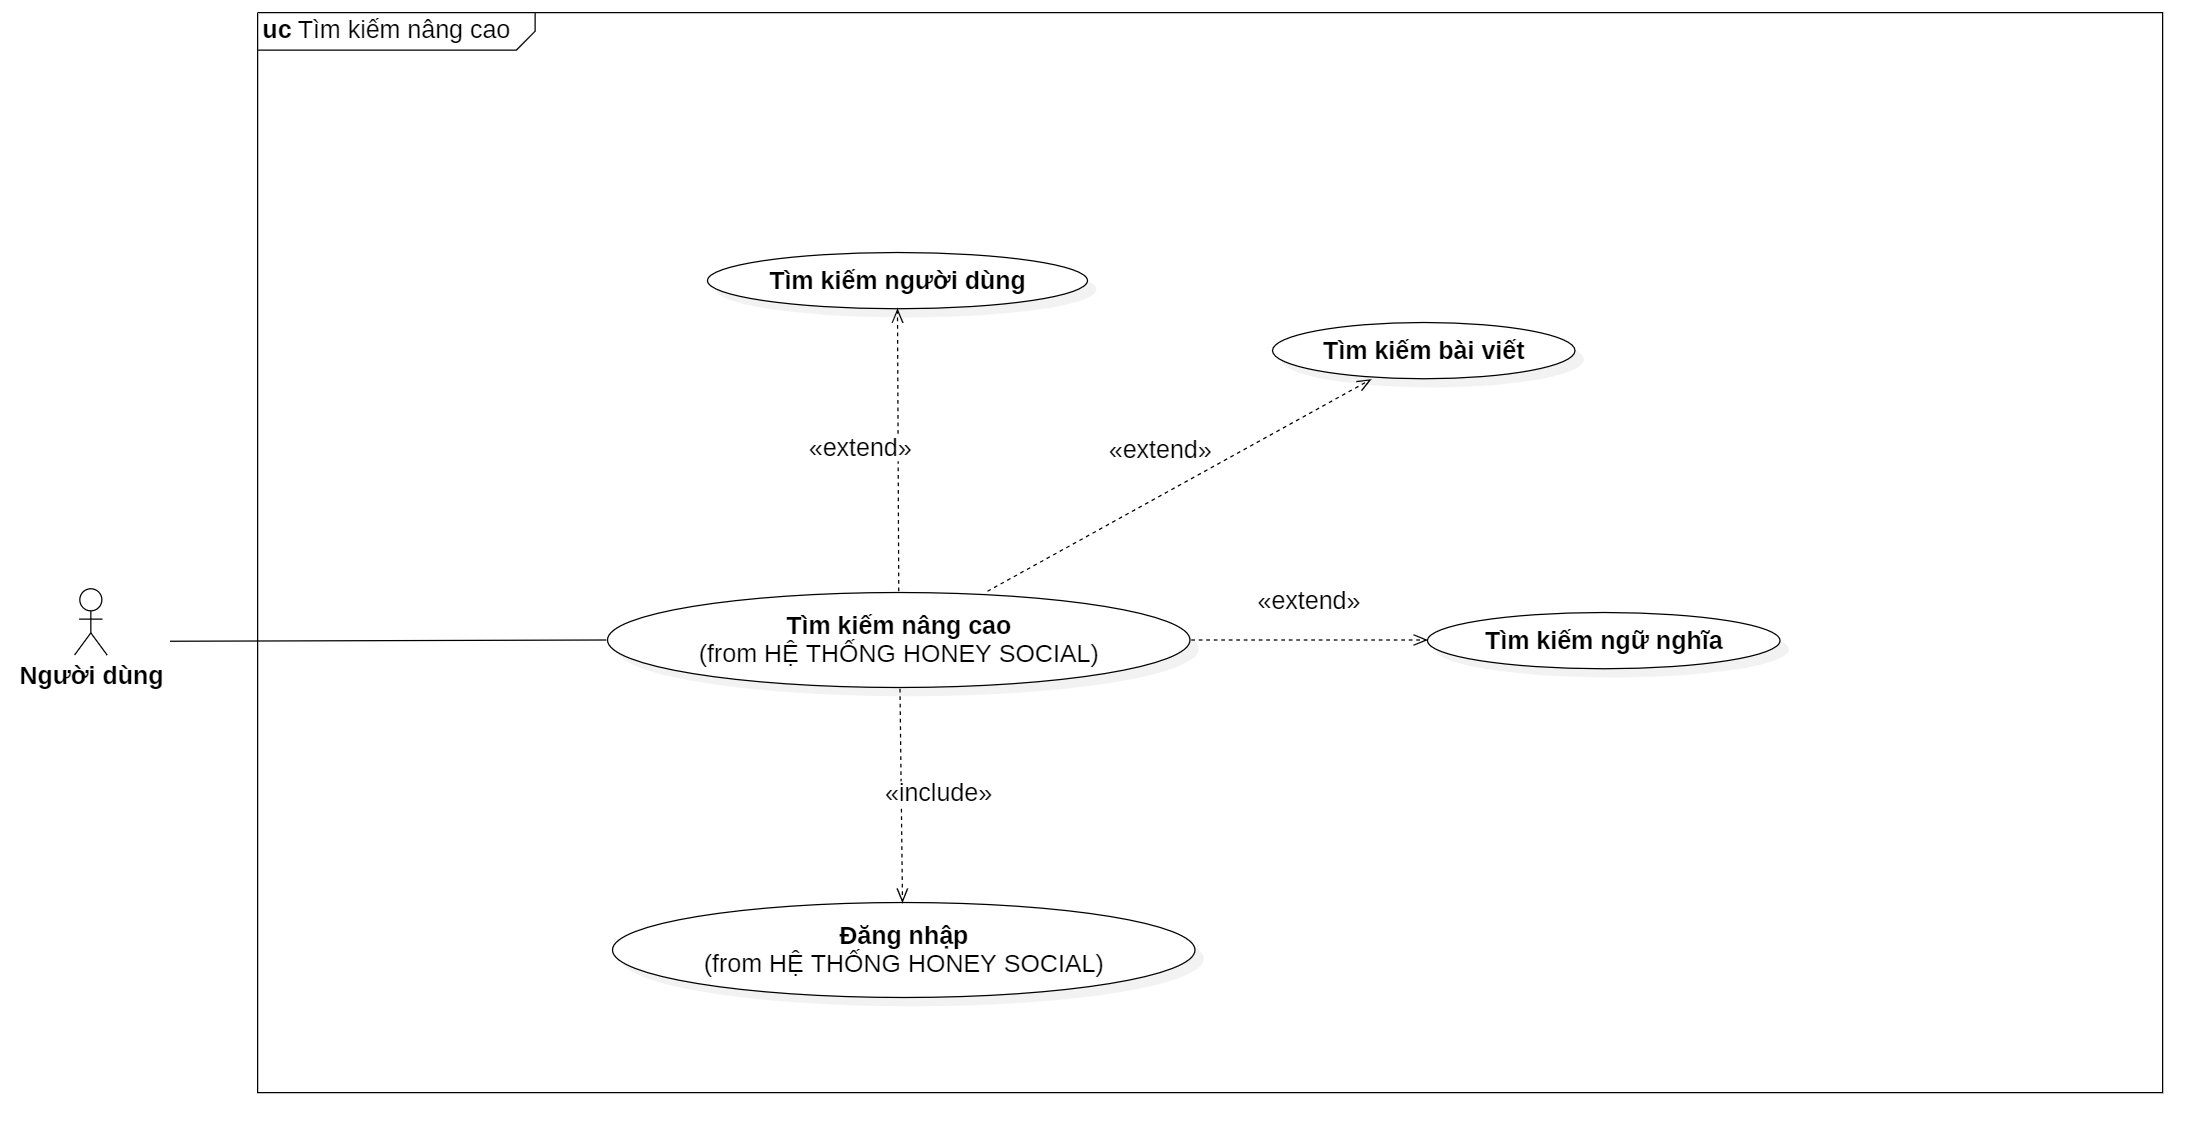
\includegraphics[width=1\textwidth]{image/MoHinh/3.png}
    \caption{Hình ảnh Tìm kiếm nâng cao}
    \label{fig:tim_kiem_nang_cao}
\end{figure}
Hiển thị quy trình tìm kiếm thông minh, cho phép người dùng sử dụng bộ lọc theo từ khóa, thời gian, hoặc sở thích cá nhân, tích hợp gợi ý dựa trên vector similarity từ Elasticsearch, và sắp xếp kết quả theo mức độ liên quan hoặc thời gian đăng tải để tối ưu hóa trải nghiệm tìm kiếm.

\newpage
\textbf{Thông báo} \\
\begin{figure}[H]
    \centering
    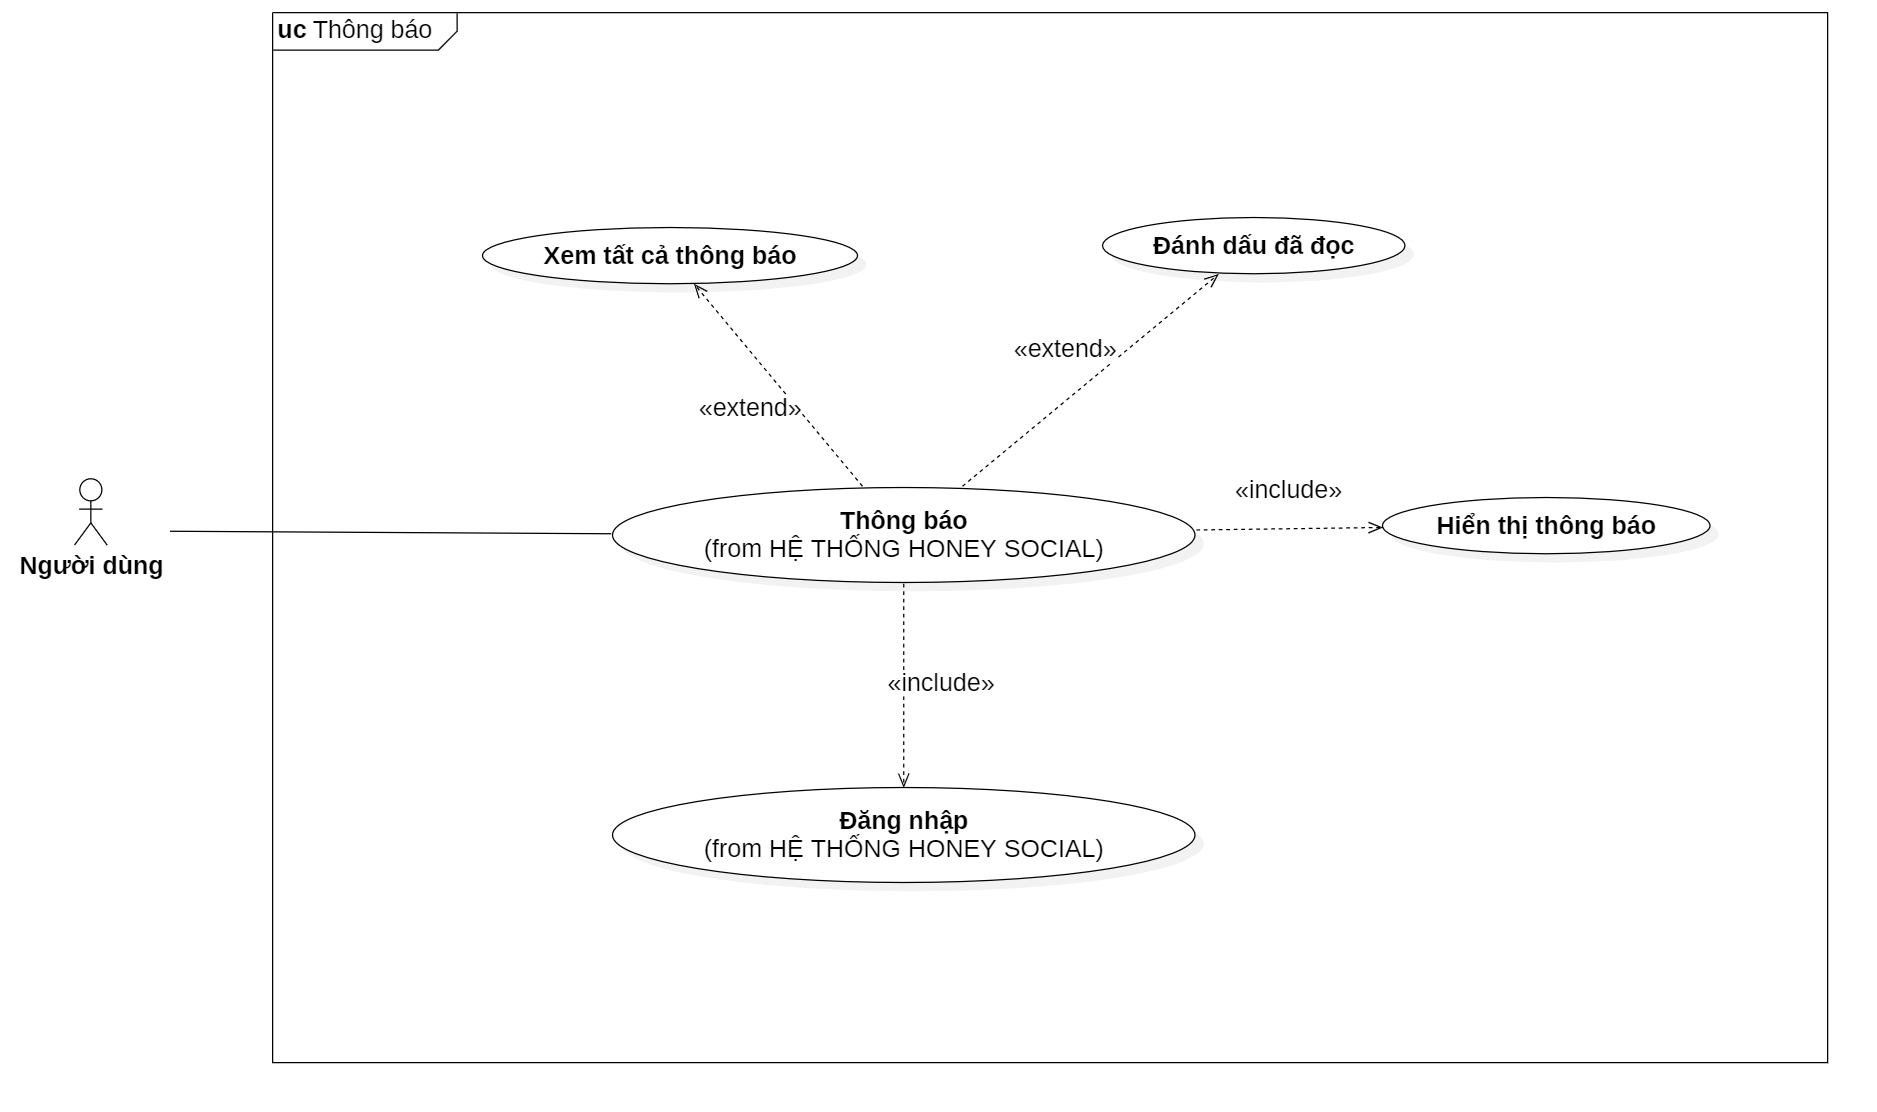
\includegraphics[width=1\textwidth]{image/MoHinh/4.png}
    \caption{Hình ảnh Thông báo}
    \label{fig:thong_bao}
\end{figure}
Chi tiết hóa cách hệ thống gửi thông báo thời gian thực, bao gồm thông báo khi có tương tác (thích, bình luận), cập nhật từ người theo dõi, hoặc thông báo hệ thống (như xác nhận email), với tùy chọn tắt/mở thông báo để cá nhân hóa trải nghiệm.

\newpage
\textbf{Xem hồ sơ người dùng} \\
\begin{figure}[H]
    \centering
    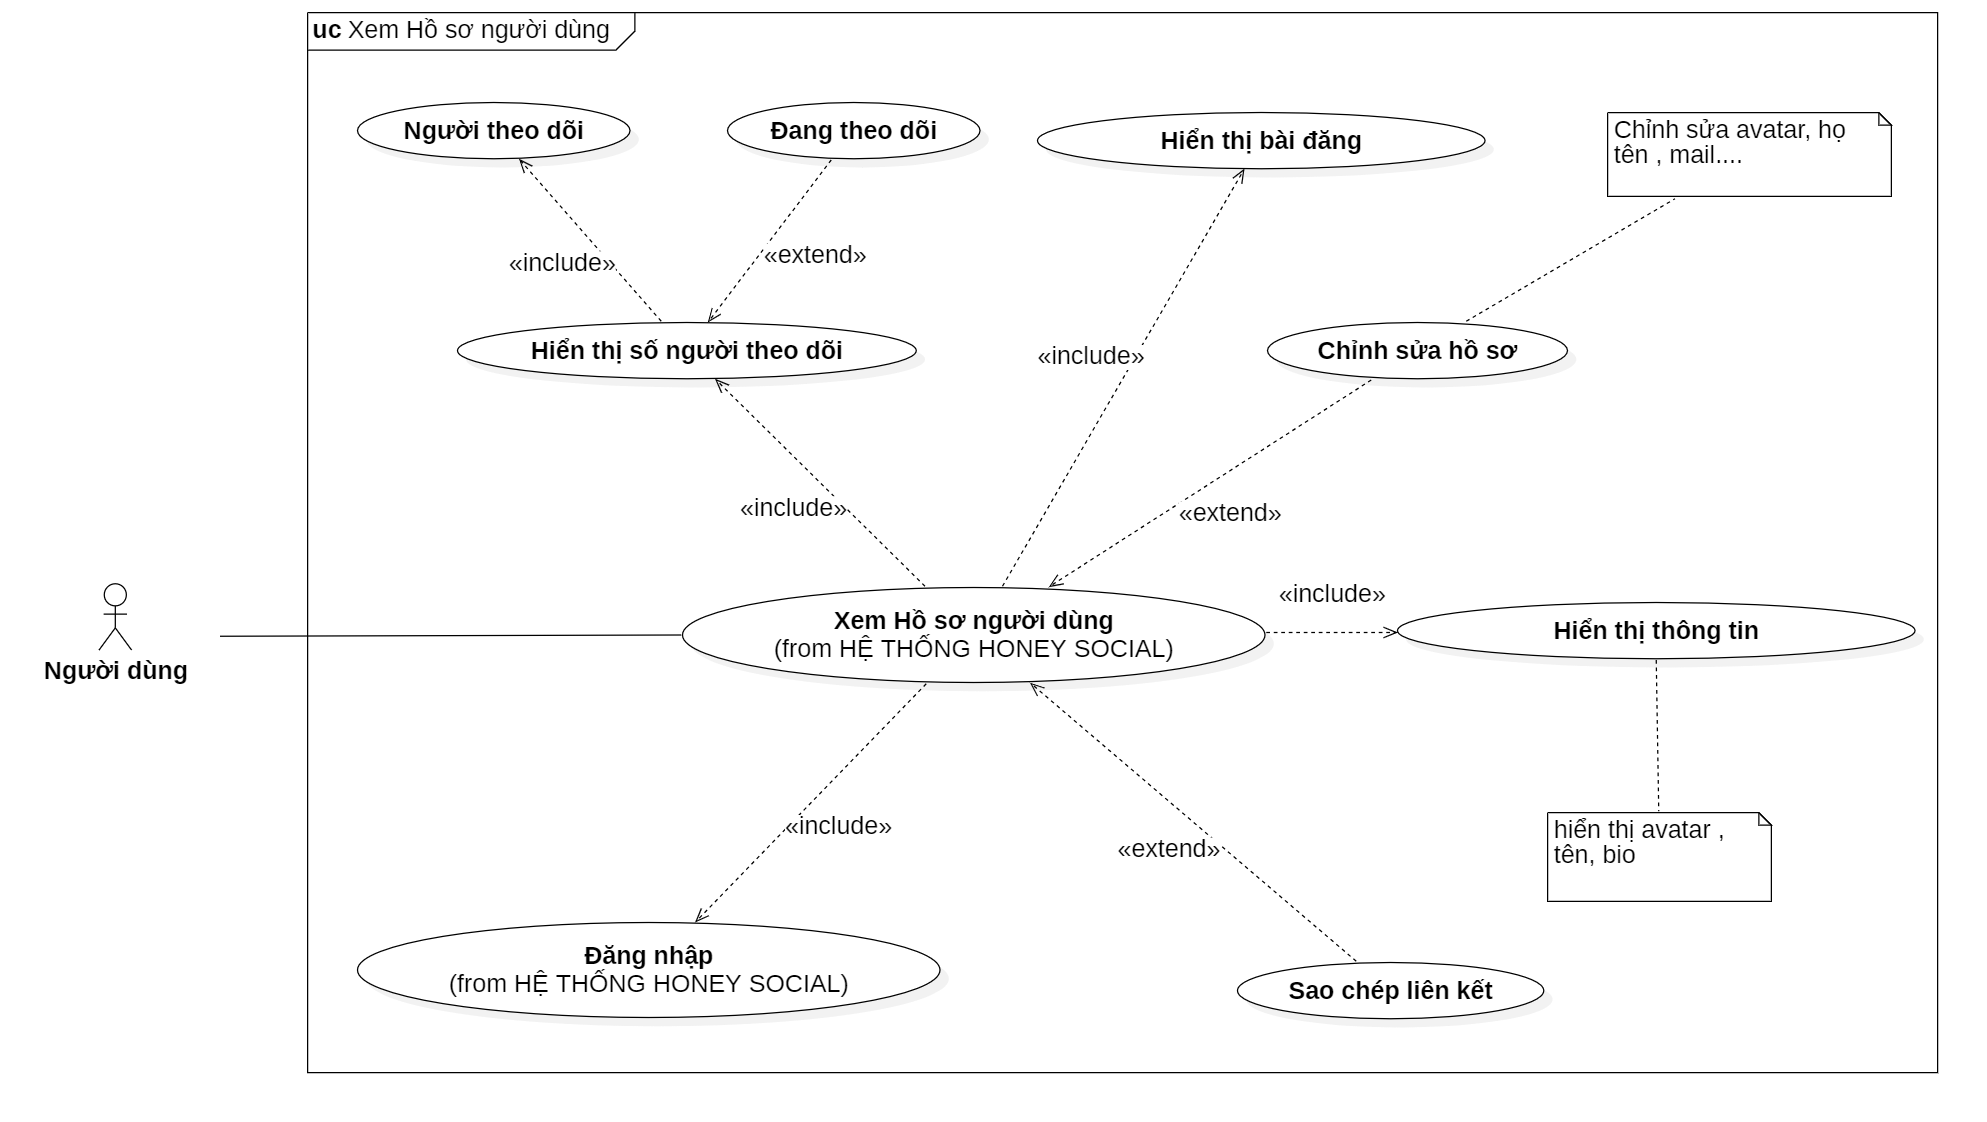
\includegraphics[width=1\textwidth]{image/MoHinh/5.png}
    \caption{Hình ảnh Xem Hồ sơ người dùng}
    \label{fig:xem_ho_so_nguoi_dung}
\end{figure}
Hướng dẫn chi tiết cách người dùng xem và chỉnh sửa hồ sơ cá nhân, bao gồm cập nhật avatar thông qua Cloudinary, chỉnh sửa thông tin như tên, bio, và danh sách theo dõi/người theo dõi, cùng với các thống kê cơ bản như số bài đăng.

\textbf{Báo cáo bài viết} \\
\begin{figure}[H]
    \centering
    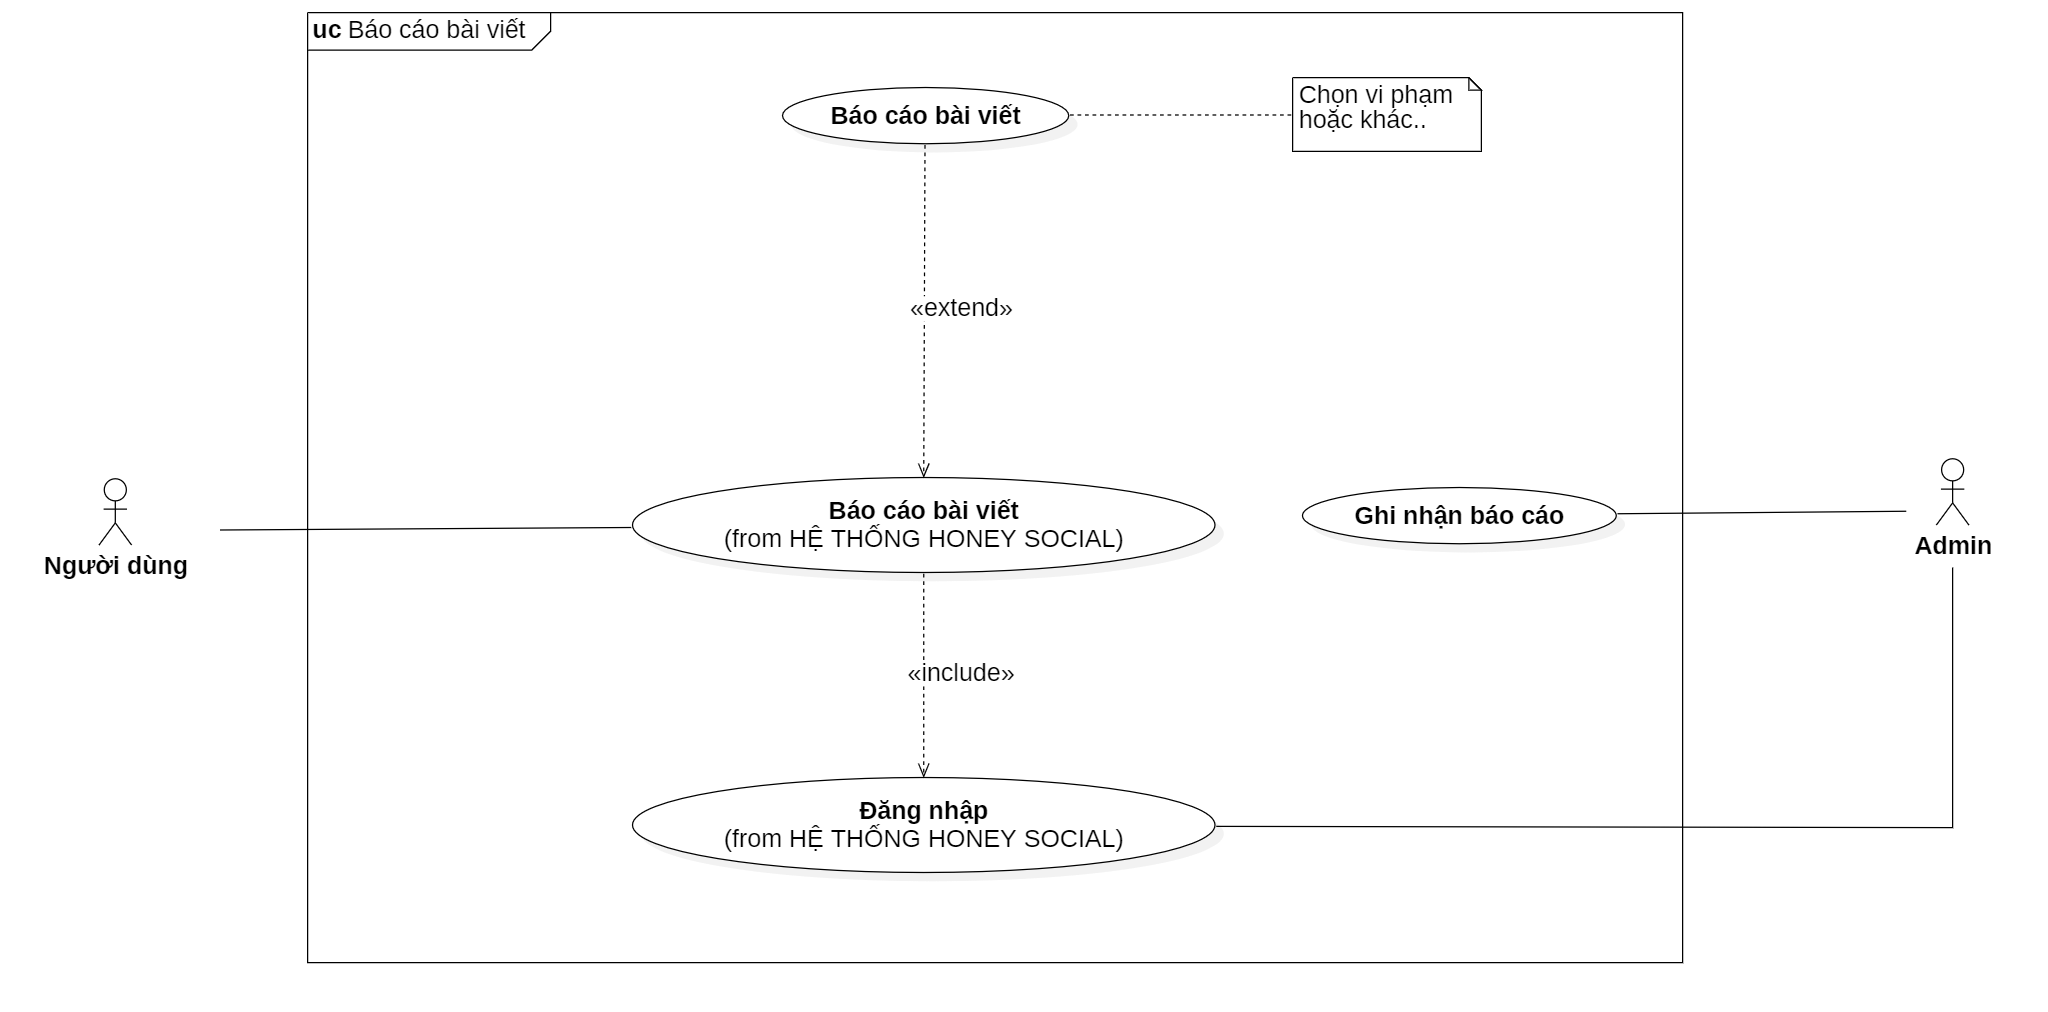
\includegraphics[width=1\textwidth]{image/MoHinh/6.png}
    \caption{Hình ảnh Báo cáo bài viết}
    \label{fig:bao_cao_bai_viet}
\end{figure}
Mô tả quy trình người dùng báo cáo vi phạm, bao gồm chọn lý do cụ thể (nội dung không phù hợp, bạo lực, spam...), gửi thông tin kèm bằng chứng qua API, và chuyển đến quản trị viên để xử lý theo các cấp độ (nhẹ, vừa, nặng).

\textbf{Trò chuyện AI} \\
\begin{figure}[H]
    \centering
    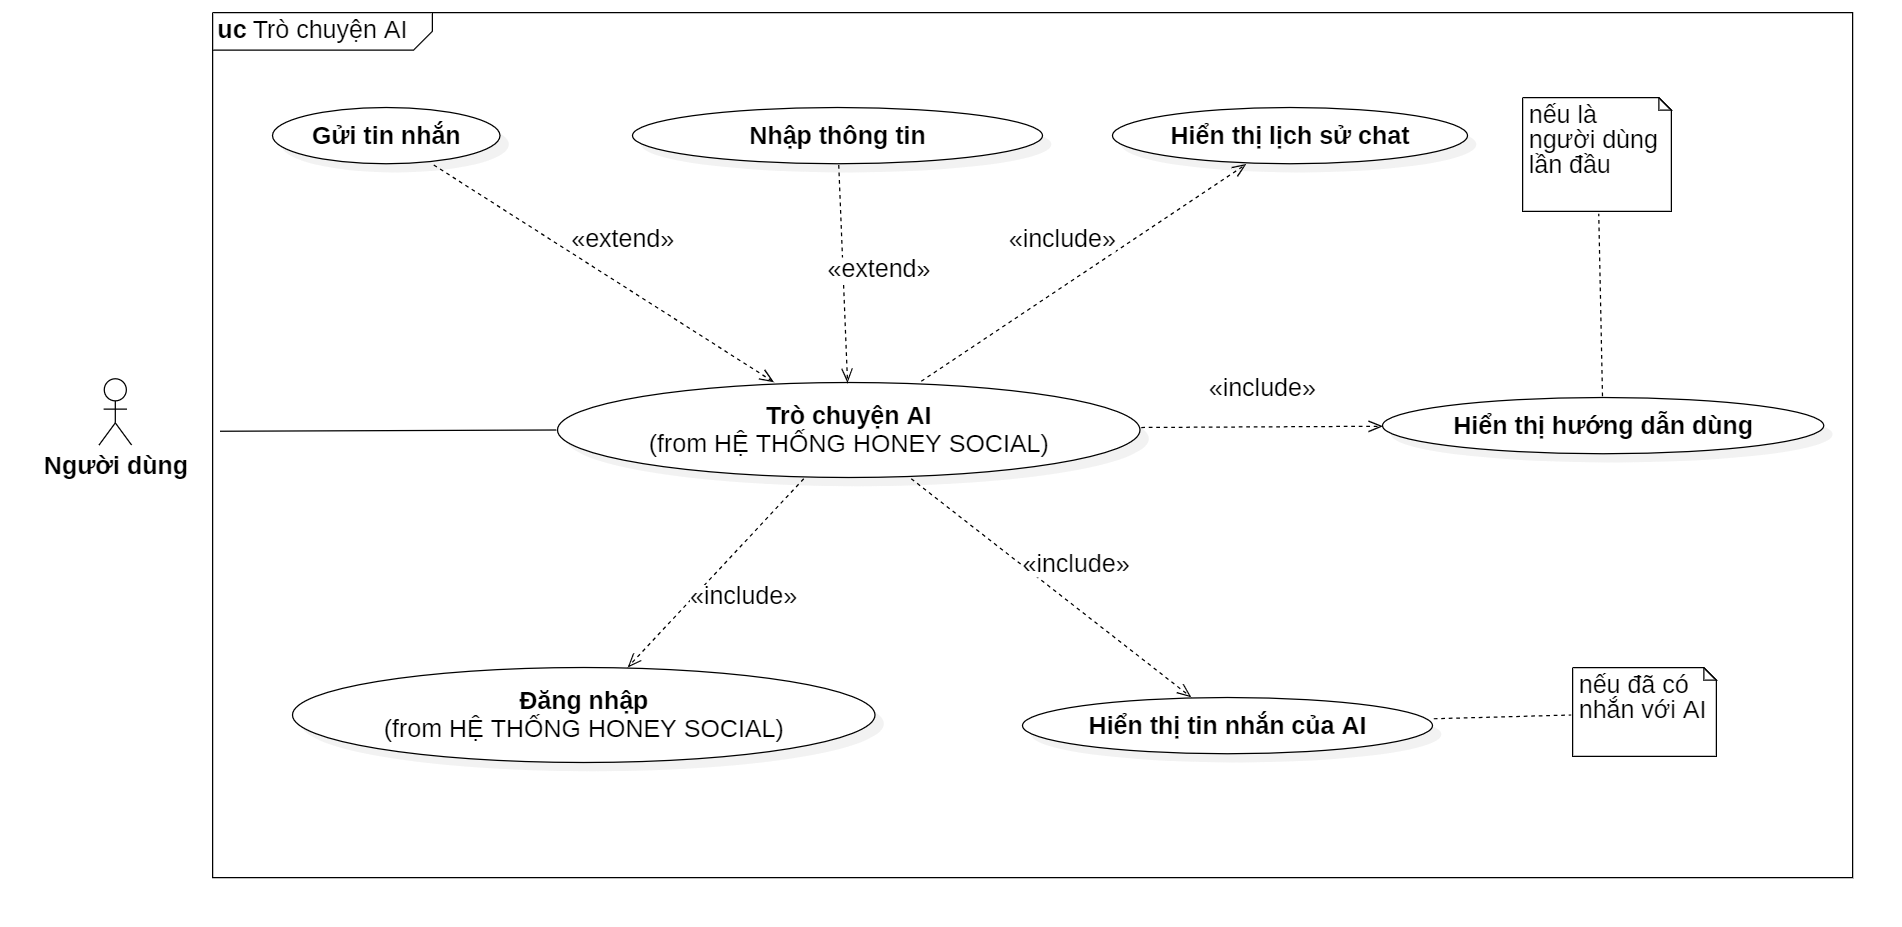
\includegraphics[width=1\textwidth]{image/MoHinh/7.png}
    \caption{Hình ảnh Trò chuyện AI}
    \label{fig:tro_chuyen_ai}
\end{figure}
Phác thảo chức năng chat AI, hỗ trợ trả lời câu hỏi liên quan đến nội dung bài viết, gợi ý bài viết dựa trên sở thích, và tự động phát hiện/phân loại báo cáo vi phạm, với giao diện thân thiện và phản hồi thời gian thực.

\newpage
\textbf{Xem bảng tin} \\
\begin{figure}[H]
    \centering
    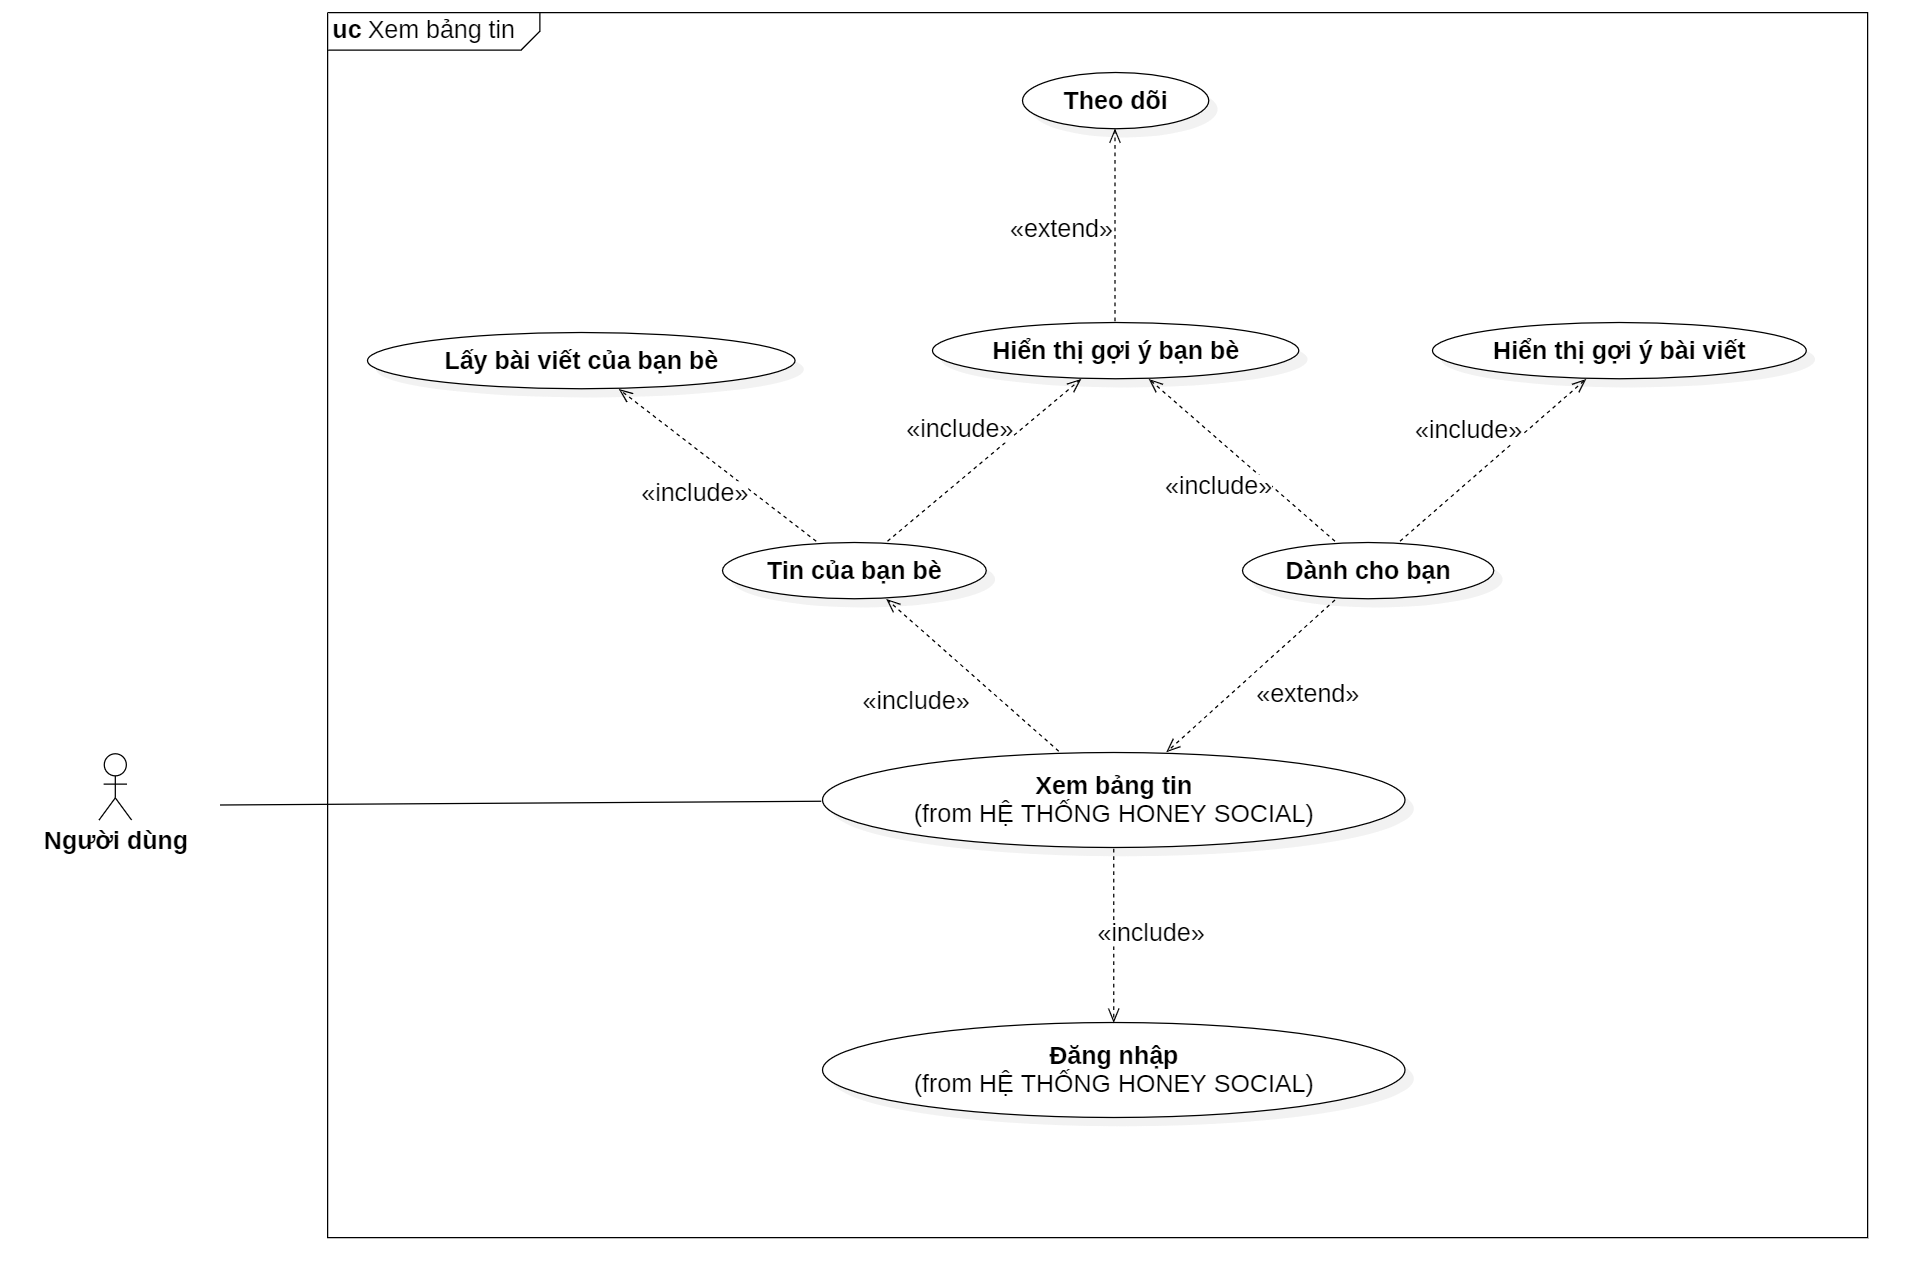
\includegraphics[width=1\textwidth]{image/MoHinh/8.png}
    \caption{Hình ảnh Xem bảng tin}
    \label{fig:xem_bang_tin}
\end{figure}
Thể hiện cách hệ thống hiển thị feed bài viết cá nhân hóa, lấy dữ liệu từ người dùng theo dõi, tích hợp gợi ý từ AI dựa trên vector nhúng, và cho phép làm mới feed hoặc lọc theo chủ đề để tăng tính tương tác.

\textbf{Xem hồ sơ người khác} \\
\begin{figure}[H]
    \centering
    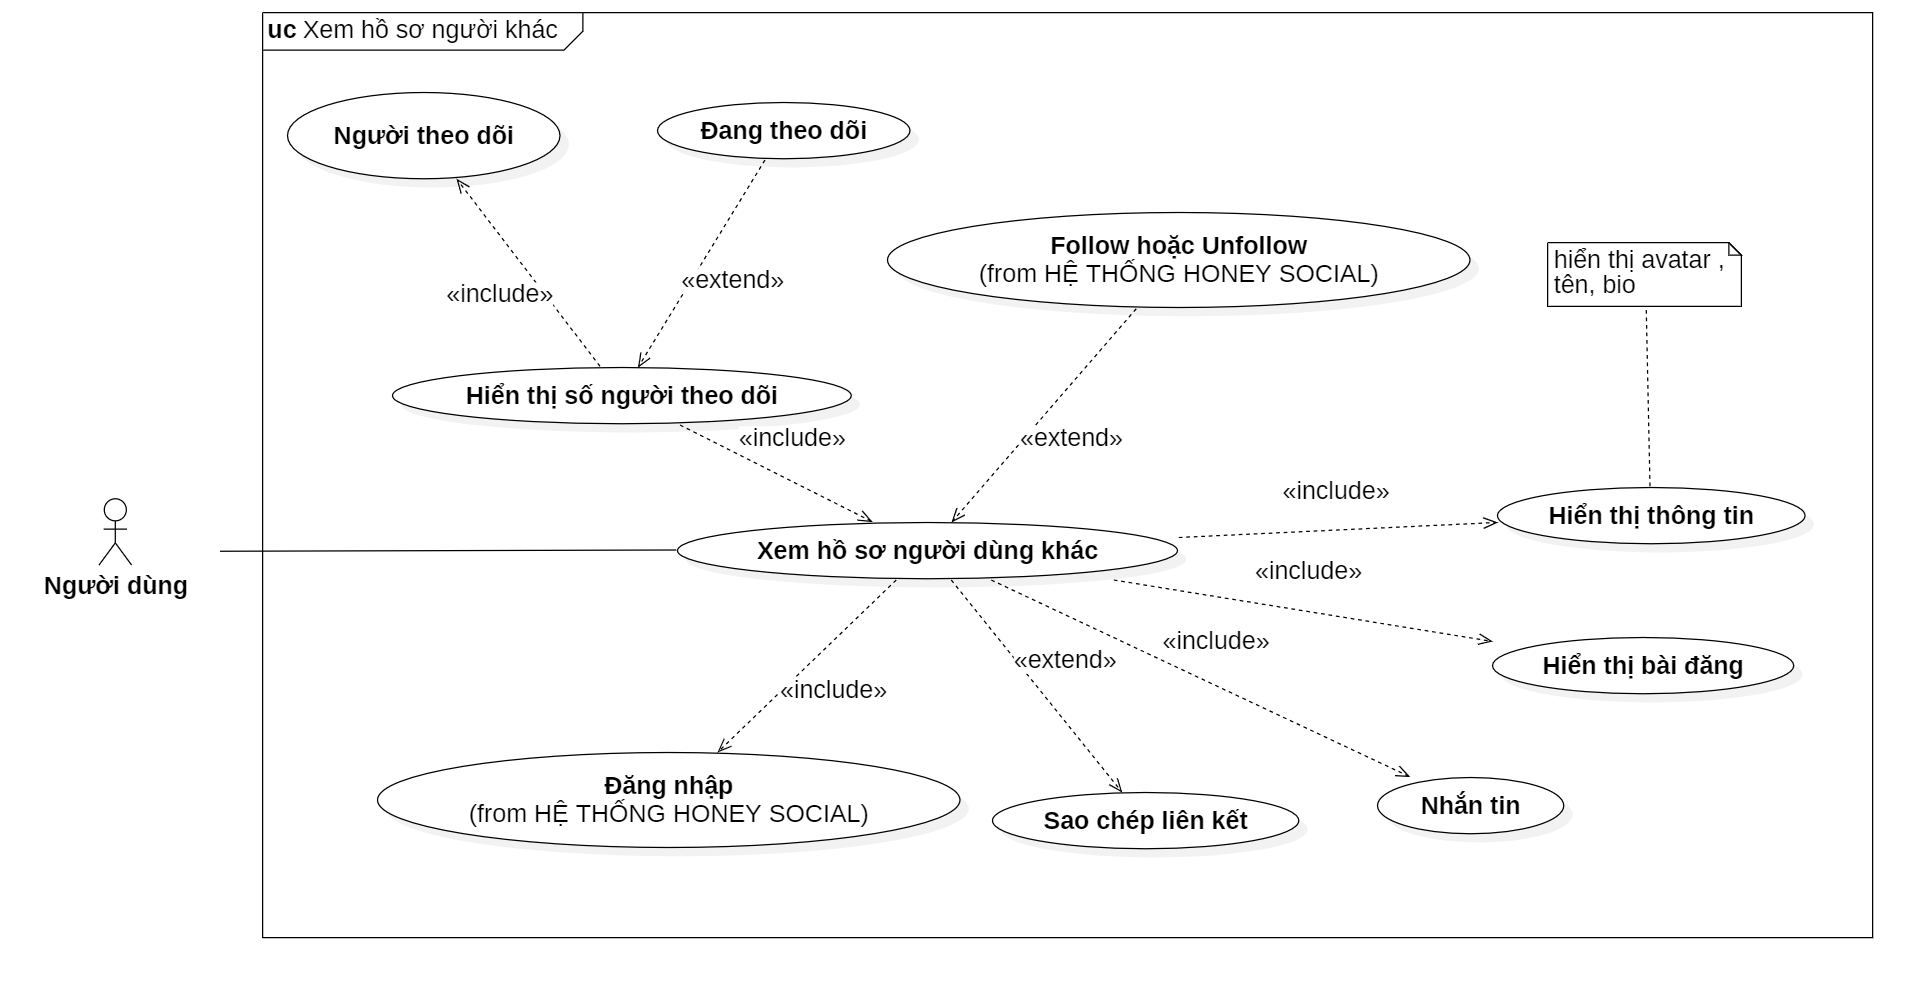
\includegraphics[width=1\textwidth]{image/MoHinh/9.png}
    \caption{Hình ảnh Xem hồ sơ người khác}
    \label{fig:xem_ho_so_nguoi_khac}
\end{figure}
Chi tiết quy trình xem hồ sơ người dùng khác, bao gồm thông tin cơ bản (tên, avatar, bio), danh sách bài đăng công khai, và các tùy chọn tương tác như theo dõi hoặc gửi tin nhắn.

\textbf{Đăng ký} \\
\begin{figure}[H]
    \centering
    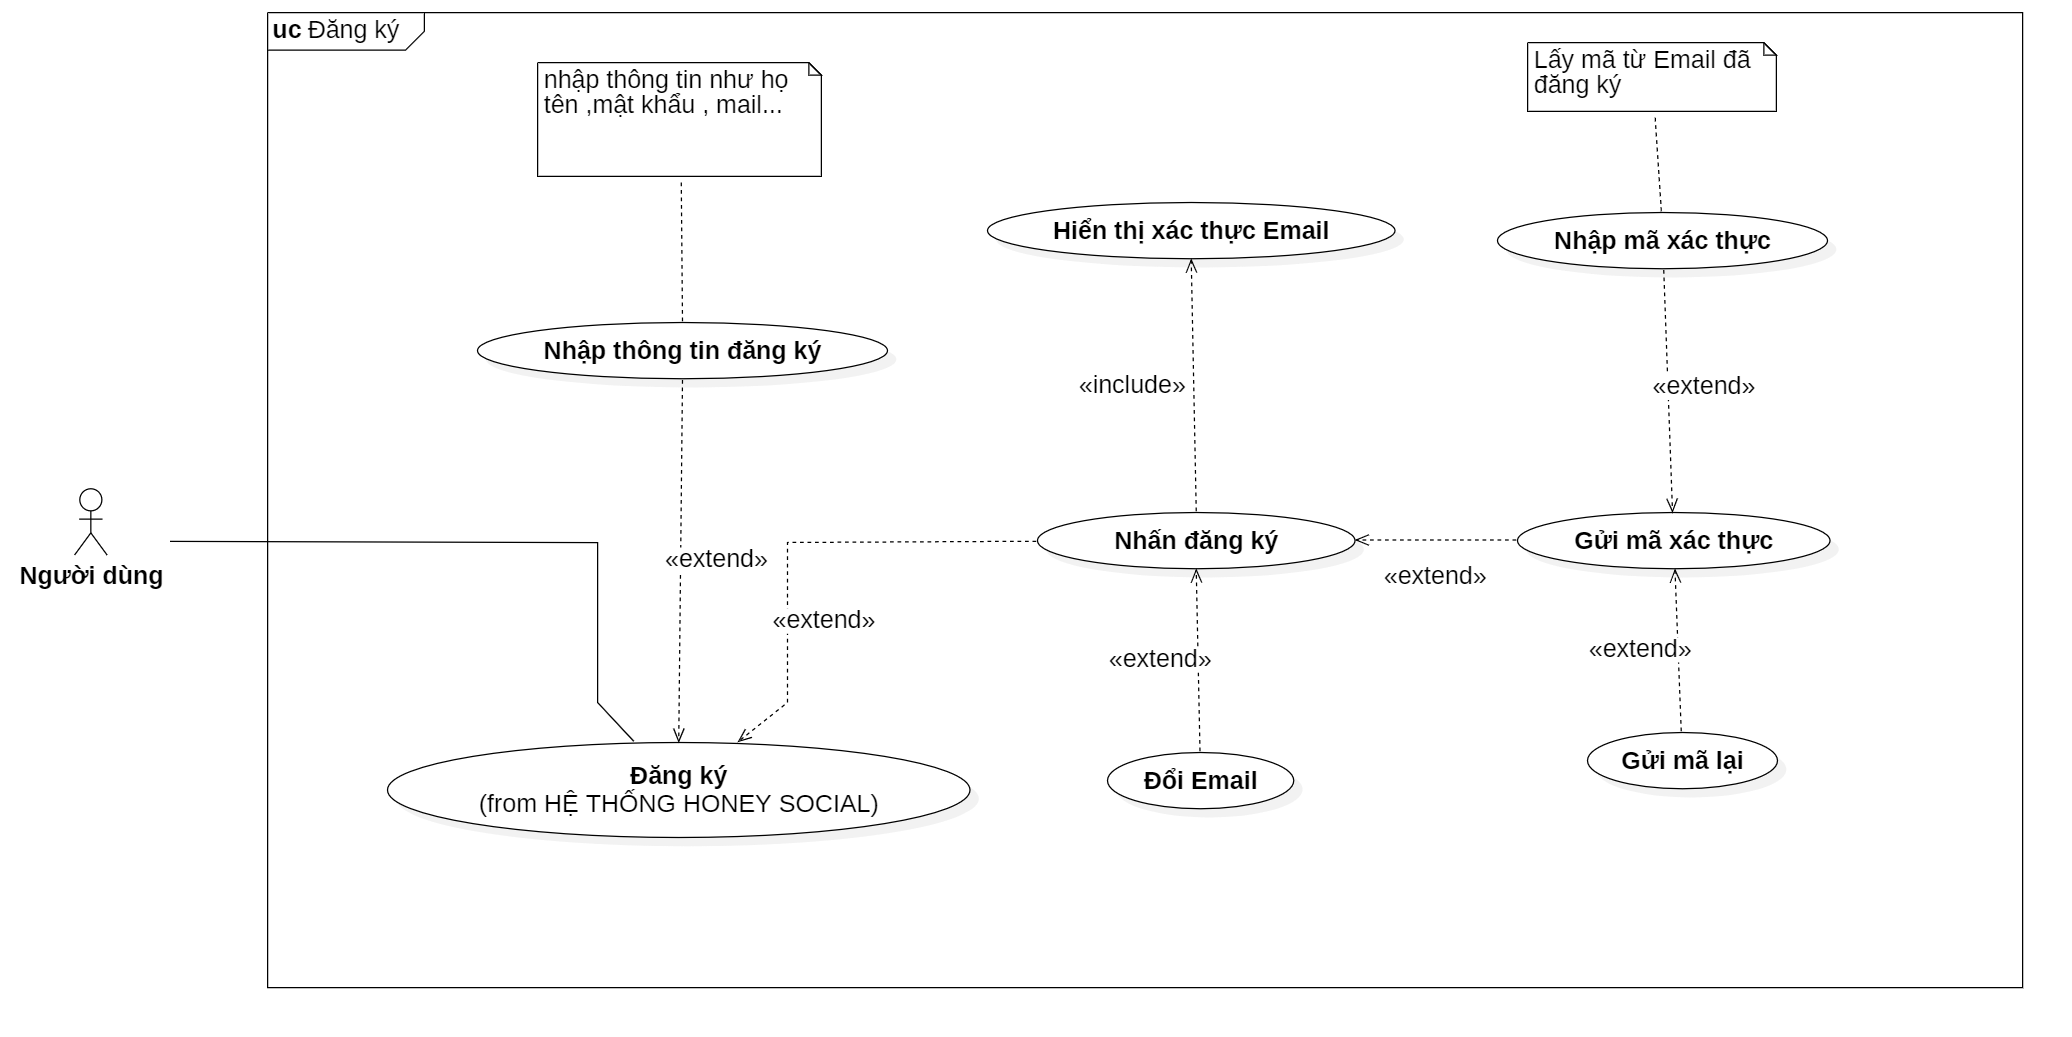
\includegraphics[width=1\textwidth]{image/MoHinh/10.png}
    \caption{Hình ảnh Đăng ký}
    \label{fig:dang_ky}
\end{figure}
Mô tả quy trình đăng ký tài khoản, yêu cầu nhập thông tin (email, mật khẩu), gửi mã OTP qua Resend API để xác thực, và hoàn tất với tùy chọn cá nhân hóa hồ sơ ngay sau đăng ký.
\newpage
\textbf{Quản lý nội dung báo cáo} \\
\begin{figure}[H]
    \centering
    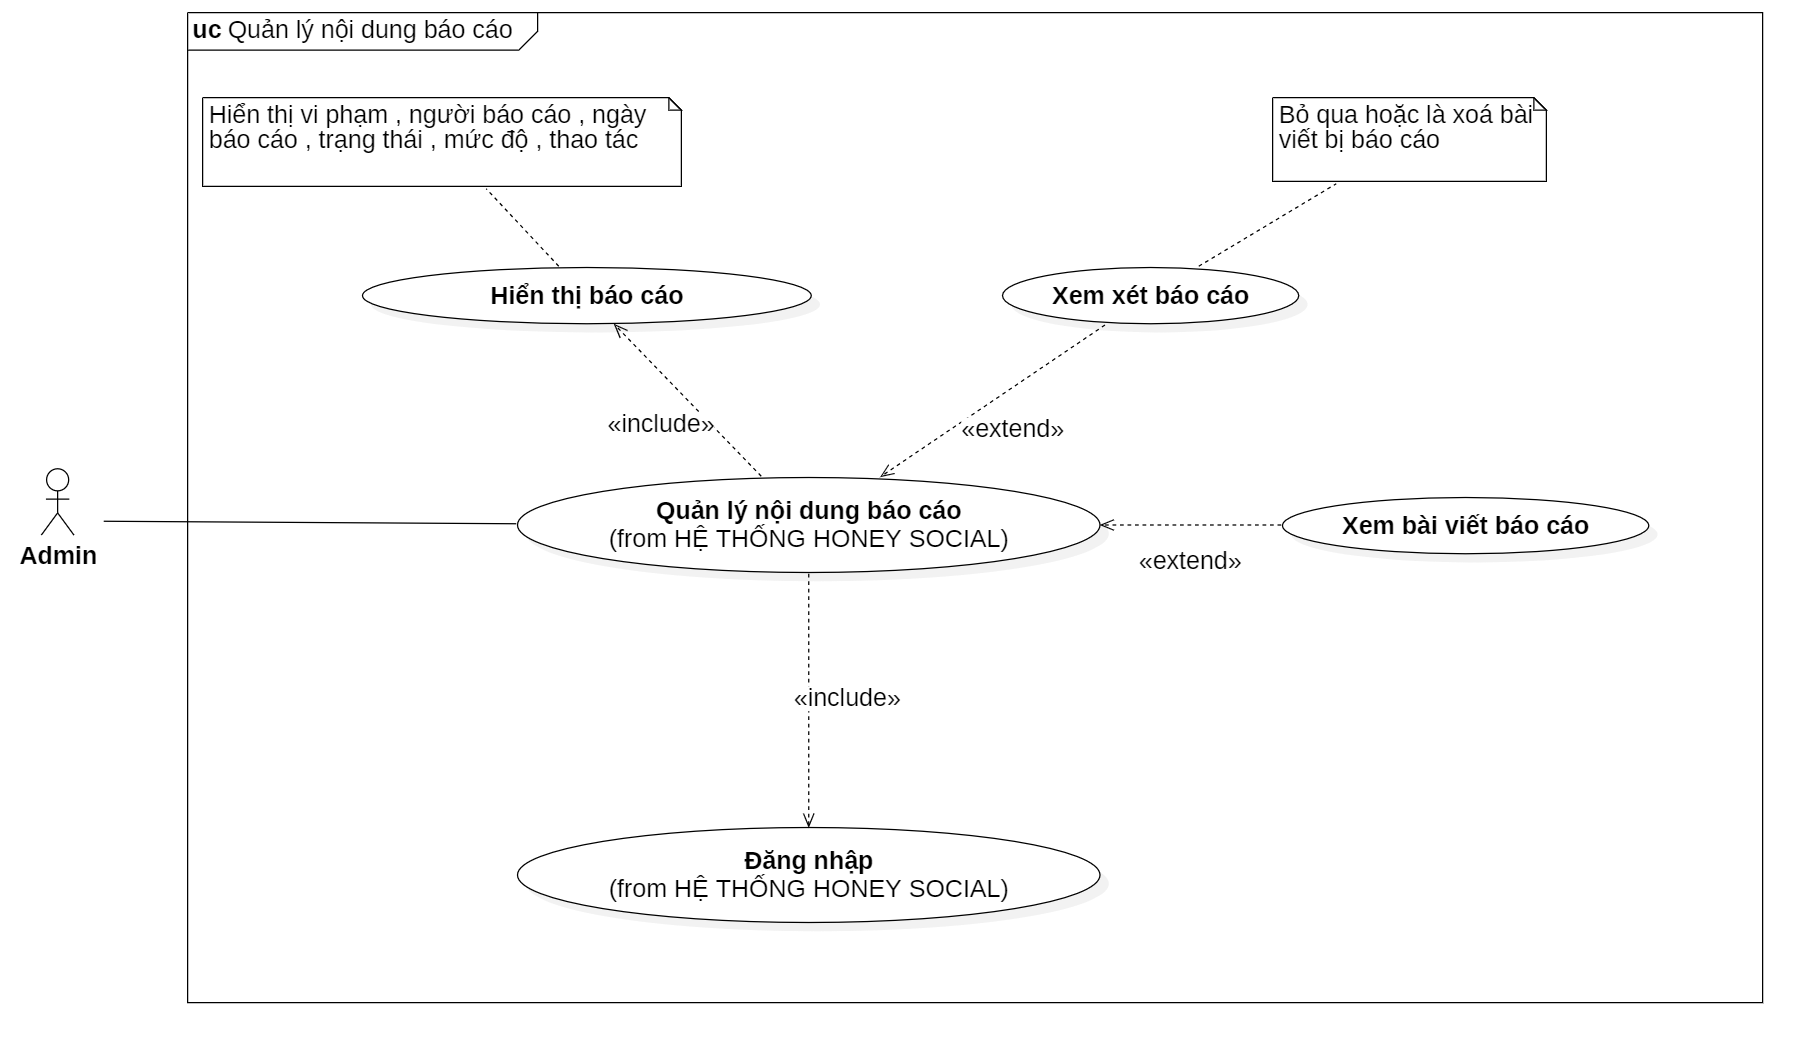
\includegraphics[width=1\textwidth]{image/MoHinh/11.png}
    \caption{Hình ảnh Quản lý nội dung báo cáo}
    \label{fig:quan_ly_noi_dung_bao_cao}
\end{figure}
Hiển thị cách quản trị viên tiếp nhận báo cáo từ người dùng, phân loại theo mức độ vi phạm (nhẹ: cảnh báo; vừa: ẩn bài; nặng: xóa và khóa tài khoản), và xử lý qua dashboard admin với các công cụ lọc theo thời gian hoặc lý do.
\newpage
\textbf{Tương tác bài viết} \\
\begin{figure}[H]
    \centering
    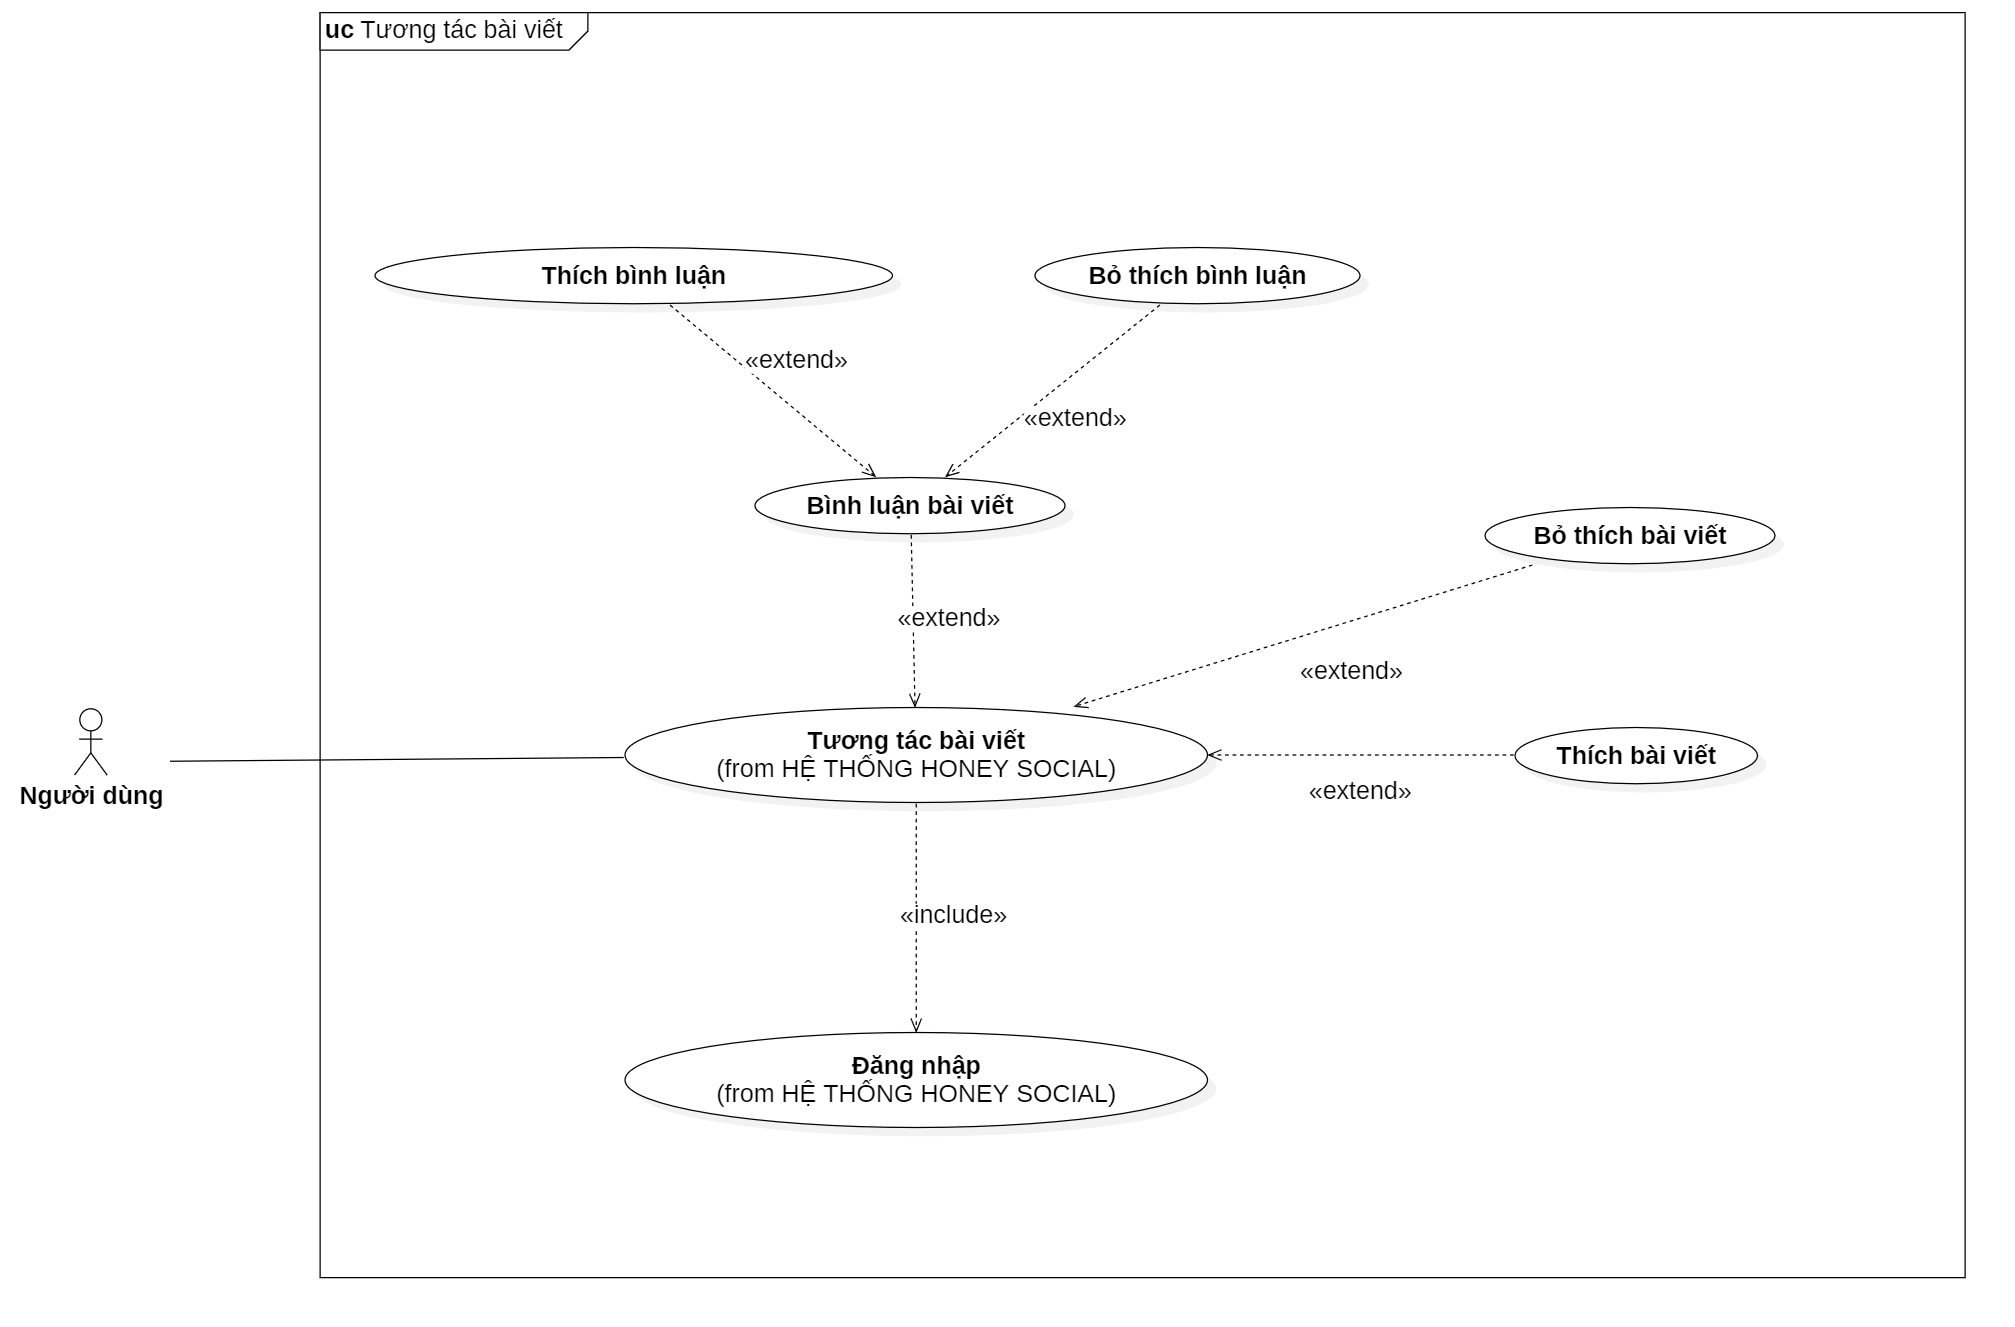
\includegraphics[width=1\textwidth]{image/MoHinh/12.png}
    \caption{Hình ảnh Tương tác bài viết}
    \label{fig:tuong_tac_bai_viet}
\end{figure}
Phác thảo các hành động tương tác như thích (like), bình luận (với khả năng phản hồi), và chia sẻ liên kết bài viết ra ngoài, tất cả đều được xử lý qua Socket.IO để đảm bảo cập nhật thời gian thực.

\newpage

\subsubsection{Kịch bản của các UseCase}


\begin{longtable}{|>{\bfseries}m{4cm}|m{10cm}|}
\caption{Bảng thông tin hoạt động của chức năng đăng bài viết}
\label{table:usecase-posts}\\
\hline
Use-case name & Đăng bài viết \\ 
\hline 
Description & Người dùng đăng một bài viết mới lên hệ thống, có thể kèm hình ảnh.\\
\hline
Actor & Người dùng đã đăng nhập\\
\hline
Pre-Conditions & -Người dùng đã đăng nhập vào hệ thống.

-Email của người dùng đã được xác thực (nếu hệ thống yêu cầu).\\
\hline
Post-Condition & -Bài viết mới được lưu vào hệ thống và hiển thị trên bảng tin.

-Nếu có lỗi, thông báo lỗi được hiển thị cho người dùng.\\
\hline
Trigger & Người dùng nhấn nút "Tạo bài viết mới" hoặc biểu tượng "+".\\
\hline
Normal Flow &
\begin{enumerate}
    \item Người dùng nhấn nút "Tạo bài viết mới".
    \item Hệ thống hiển thị modal nhập nội dung bài viết.
    \item Người dùng nhập nội dung, chọn hình ảnh (nếu muốn).
    \item Người dùng nhấn nút "Đăng".
    \item Hệ thống kiểm tra điều kiện (đăng nhập, xác thực email, nội dung hợp lệ).
    \item Nếu hợp lệ, bài viết được lưu và hiển thị; thông báo thành công cho người dùng.
\end{enumerate} \\
\hline
Alternative Flow & Nếu người dùng chưa đăng nhập: Hệ thống thông báo và chuyển hướng đến trang đăng nhập.

Nếu email chưa xác thực: Hệ thống thông báo yêu cầu xác thực email.

Nếu nội dung vi phạm hoặc lỗi khác: Hệ thống hiển thị thông báo lỗi chi tiết.

Nếu người dùng nhấn "Hủy": Modal đóng, không lưu bài viết.\\
\hline
\end{longtable}


% \subsubsubsection{Chức năng tìm kiếm nâng cao}
\begin{longtable}{|>{\bfseries}m{4cm}|m{10cm}|}
\caption{Bảng thông tin hoạt động của chức năng tìm kiếm nâng cao}
\label{table:usecase-search}\\
\hline
Use-case name & Tìm kiếm nâng cao
\\
\hline
Description & Người dùng thực hiện tìm kiếm nâng cao để tìm kiếm người dùng, bài viết hoặc theo ngữ nghĩa trên hệ thống.\\
\hline
Actor & Người dùng đã đăng nhập
\\
\hline
Pre-Conditions & Người dùng đã đăng nhập vào hệ thống.

Hệ thống có dữ liệu người dùng/bài viết.\\
\hline
Post-Condition & Kết quả tìm kiếm được hiển thị cho người dùng theo tiêu chí đã chọn.

Người dùng có thể chuyển trang, sắp xếp hoặc chọn kết quả để xem chi tiết.\\
\hline
Trigger & Người dùng truy cập trang tìm kiếm nâng cao hoặc nhập từ khóa vào ô tìm kiếm.
\\
\hline
Normal Flow &
\begin{enumerate}
    \item Người dùng truy cập chức năng tìm kiếm nâng cao.
    \item Người dùng nhập từ khóa tìm kiếm.
    \item Hệ thống gửi yêu cầu tìm kiếm đến server với từ khóa và các tham số (phân trang, sắp xếp).
    \item Server xử lý và trả về danh sách kết quả phù hợp.
    \item Hệ thống hiển thị kết quả tìm kiếm cho người dùng, kèm số lượng và các tuỳ chọn sắp xếp.
    \item Người dùng có thể chuyển trang, thay đổi tiêu chí sắp xếp hoặc nhấn vào kết quả để xem chi tiết.
\end{enumerate} \\
\hline
Alternative Flow & Nếu người dùng chưa đăng nhập: Hệ thống yêu cầu đăng nhập trước khi sử dụng tìm kiếm nâng cao.


Nếu không có kết quả phù hợp: Hệ thống hiển thị thông báo "Không tìm thấy người dùng phù hợp".


Nếu xảy ra lỗi server hoặc kết nối: Hệ thống hiển thị thông báo lỗi cho người dùng.\\
\hline
\end{longtable}

% \subsubsubsection{Chức năng thông báo}
\begin{longtable}{|>{\bfseries}m{4cm}|m{10cm}|}
\caption{Bảng thông tin hoạt động của chức năng thông báo}
\label{table:usecase-noti}\\
\hline

Use-case name & Thông báo
\\
\hline
Description & Người dùng xem danh sách thông báo, đánh dấu thông báo đã đọc hoặc xem chi tiết thông báo.\\
\hline
Actor & Người dùng đã đăng nhập\\
\hline
Pre-Conditions & Người dùng đã đăng nhập vào hệ thống.

Hệ thống có thông báo liên quan đến người dùng.\\
\hline
Post-Condition & Thông báo được hiển thị cho người dùng.

Thông báo được đánh dấu là đã đọc (nếu người dùng thực hiện hành động này).\\
\hline
Trigger & Người dùng nhấn vào biểu tượng thông báo trên giao diện.\\
\hline
Normal Flow &
\begin{enumerate}
    \item Người dùng nhấn vào biểu tượng thông báo.
    \item Hệ thống hiển thị danh sách thông báo.
    \item Người dùng chọn một thông báo để xem chi tiết.
    \item Hệ thống đánh dấu thông báo đã đọc và hiển thị nội dung chi tiết.
    \item Người dùng quay lại danh sách thông báo hoặc tiếp tục sử dụng hệ thống.
\end{enumerate} \\
\hline
Alternative Flow & Nếu không có thông báo: Hệ thống hiển thị thông báo "Không có thông báo mới".

Nếu người dùng chưa đăng nhập: Hệ thống yêu cầu người dùng đăng nhập để xem thông báo.\\
\hline
\end{longtable}

% \subsubsubsection{Chức năng xem hồ sơ người dùng}

\begin{longtable}{|>{\bfseries}m{4cm}|m{10cm}|}
    \caption{Bảng thông tin hoạt động của chức năng xem hồ sơ người dùng}
    \label{table:usecase-profile}\\
    
\hline
Use-case name & Xem hồ sơ người dùng \\
\hline
Description & Người dùng có thể xem hồ sơ của bản thân hoặc người dùng khác, bao gồm thông tin cá nhân, danh sách bài đăng, số lượng người theo dõi và đang theo dõi. \\
\hline
Actor & Người dùng đã đăng nhập \\
\hline
Pre-Conditions & 
\begin{itemize}
    \item Người dùng đã đăng nhập vào hệ thống.
    \item Hồ sơ của người dùng hoặc người khác tồn tại trong hệ thống.
\end{itemize} \\
\hline
Post-Condition & 
\begin{itemize}
    \item Hồ sơ người dùng được hiển thị đầy đủ thông tin.
    \item Người dùng có thể thực hiện các hành động như theo dõi, nhắn tin, hoặc chỉnh sửa hồ sơ (nếu là hồ sơ của chính họ).
\end{itemize} \\
\hline
Trigger & Người dùng nhấn vào tên hoặc ảnh đại diện của một người dùng khác hoặc chọn mục "Hồ sơ" từ menu cá nhân. \\
\hline
Normal Flow &
\begin{enumerate}
    \item Người dùng nhấn vào tên hoặc ảnh đại diện của một người dùng khác hoặc chọn mục "Hồ sơ".
    \item Hệ thống kiểm tra quyền truy cập và tải thông tin hồ sơ từ cơ sở dữ liệu.
    \item Hệ thống hiển thị thông tin cá nhân (tên, ảnh đại diện, tiểu sử, v.v.).
    \item Hệ thống hiển thị danh sách bài đăng của người dùng.
    \item Hệ thống hiển thị số lượng người theo dõi và đang theo dõi.
    \item Người dùng có thể thực hiện các hành động như theo dõi, nhắn tin, hoặc chỉnh sửa hồ sơ (nếu là hồ sơ của chính họ).
\end{enumerate} \\
\hline
Alternative Flow & 
\begin{itemize}
    \item Nếu người dùng chưa đăng nhập: Hệ thống yêu cầu đăng nhập trước khi xem hồ sơ.
    \item Nếu hồ sơ không tồn tại: Hệ thống hiển thị thông báo lỗi "Hồ sơ không tồn tại".
    \item Nếu xảy ra lỗi kết nối: Hệ thống hiển thị thông báo lỗi và yêu cầu thử lại.
\end{itemize} \\
\hline
\end{longtable}


% \subsubsubsection{Chức năng báo cáo bài viết}
\begin{longtable}{|>{\bfseries}m{4cm}|m{10cm}|}
    \caption{Bảng thông tin hoạt động của chức năng báo cáo bài viết}
    \label{table:usecase-report}\\
\hline
Use-case name & Báo cáo bài viết \\
\hline
Description & Người dùng báo cáo một bài viết vi phạm các quy định của cộng đồng. \\
\hline
Actor & Người dùng đã đăng nhập \\
\hline
Pre-Conditions & 
\begin{itemize}
    \item Người dùng đã đăng nhập.
    \item Bài viết tồn tại và được hiển thị trên giao diện.
\end{itemize} \\
\hline
Post-Condition & 
\begin{itemize}
    \item Báo cáo được ghi nhận và gửi đến bộ phận kiểm duyệt.
    \item Bài viết có thể bị ẩn khỏi người dùng báo cáo (tùy thuộc vào cài đặt).
\end{itemize} \\
\hline
Trigger & Người dùng chọn tùy chọn "Báo cáo bài viết" từ menu tương tác của bài viết. \\
\hline
Normal Flow &
\begin{enumerate}
    \item Người dùng nhấn vào menu “More options” của bài viết.
    \item Hệ thống hiển thị danh sách các tùy chọn tương tác.
    \item Người dùng chọn "Báo cáo bài viết".
    \item Hệ thống hiển thị hộp thoại báo cáo, cho phép chọn lý do báo cáo (ví dụ: nội dung khiêu dâm, bạo lực, ngôn từ gây thù ghét, v.v.).
    \item Người dùng có thể nhập thêm thông tin chi tiết về lý do báo cáo (nếu cần).
    \item Người dùng nhấn nút "Gửi báo cáo".
    \item Hệ thống gửi thông tin báo cáo đến server.
    \item Hệ thống nhận phản hồi từ server và hiển thị thông báo kết quả cho người dùng (thành công hoặc lỗi).
\end{enumerate} \\
\hline
Alternative Flow &
\begin{itemize}
    \item Nếu người dùng chưa chọn lý do báo cáo: Hệ thống yêu cầu chọn một lý do trước khi gửi.
    \item Nếu có lỗi kết nối hoặc server: Hệ thống hiển thị thông báo lỗi và yêu cầu thử lại.
\end{itemize} \\
\hline
\end{longtable}

% \subsubsubsection{Chức năng trò chuyện AI}
\begin{longtable}{|>{\bfseries}m{4cm}|m{10cm}|}
    \caption{Bảng thông tin hoạt động của chức năng trò chuyện AI}
    \label{table:usecase-chat-ai}\\
\hline
Use-case name & Trò chuyện AI \\
\hline
Description & Người dùng tương tác với trợ lý AI thông qua giao diện chat, có thể gửi tin nhắn, nhận phản hồi và xem lịch sử trò chuyện. \\
\hline
Actor & Người dùng đã đăng nhập \\
\hline
Pre-Conditions & 
\begin{itemize}
    \item Người dùng đã đăng nhập vào hệ thống.
    \item Kết nối internet hoạt động bình thường.
    \item Hệ thống AI đang hoạt động.
\end{itemize} \\
\hline
Post-Condition & 
\begin{itemize}
    \item Tin nhắn của người dùng được gửi và lưu trữ.
    \item AI phản hồi và hiển thị tin nhắn cho người dùng.
    \item Lịch sử trò chuyện được cập nhật.
\end{itemize} \\
\hline
Trigger & Người dùng truy cập tính năng Chat AI thông qua menu điều hướng hoặc biểu tượng AI Chat. \\
\hline
Normal Flow &
\begin{enumerate}
    \item Người dùng nhấn vào biểu tượng Chat AI trên thanh điều hướng (desktop) hoặc chọn "Chat với AI" từ menu chat (mobile).
    \item Hệ thống chuyển hướng đến trang chat AI (/chat).
    \item Hệ thống hiển thị giao diện chat và hướng dẫn sử dụng (nếu là lần đầu truy cập).
    \item Người dùng nhập nội dung tin nhắn vào ô văn bản.
    \item Người dùng gửi tin nhắn bằng cách nhấn nút gửi hoặc phím Enter.
    \item Hệ thống hiển thị tin nhắn của người dùng trong cửa sổ chat và gửi yêu cầu đến API AI.
    \item AI xử lý yêu cầu và gửi phản hồi.
    \item Hệ thống hiển thị phản hồi của AI trong cửa sổ chat.
\end{enumerate} \\
\hline
Alternative Flow &
\begin{itemize}
    \item Nếu người dùng chưa đăng nhập: Hệ thống yêu cầu người dùng đăng nhập trước khi sử dụng tính năng.
    \item Nếu kết nối bị gián đoạn: Hệ thống hiển thị thông báo lỗi và lưu tin nhắn để gửi lại sau.
    \item Nếu AI không thể xử lý yêu cầu: Hệ thống hiển thị thông báo lỗi phù hợp và gợi ý người dùng thử lại.
    \item Nếu người dùng tải lại trang: Hệ thống tải lại lịch sử trò chuyện từ cơ sở dữ liệu.
\end{itemize} \\
\hline
\end{longtable}

\newpage
% \subsubsubsection{Chức năng xem bảng tin}
\begin{longtable}{|>{\bfseries}m{4cm}|m{10cm}|}
    \caption{Bảng thông tin hoạt động của chức năng xem bảng tin}
    \label{table:usecase-feed}\\
\hline
Use-case name & Xem bảng tin \\
\hline
Description & Người dùng xem bảng tin chứa các bài viết từ bạn bè hoặc bài viết được gợi ý dựa trên sở thích và tương tác của họ. \\
\hline
Actor & Người dùng đã đăng nhập \\
\hline
Pre-Conditions & 
\begin{itemize}
    \item Người dùng đã đăng nhập vào hệ thống.
    \item Kết nối internet hoạt động bình thường.
\end{itemize} \\
\hline
Post-Condition & 
\begin{itemize}
    \item Người dùng xem được các bài viết trên bảng tin.
    \item Hệ thống ghi nhận các tương tác của người dùng với bảng tin.
\end{itemize} \\
\hline
Trigger & Người dùng truy cập trang chủ hoặc tính năng "Bảng tin". \\
\hline
Normal Flow &
\begin{enumerate}
    \item Người dùng truy cập trang chủ của hệ thống.
    \item Hệ thống hiển thị giao diện bảng tin với hai tab: "Tin của bạn bè" và "Dành cho bạn".
    \item Mặc định, hệ thống hiển thị tab "Tin của bạn bè" với:
      \begin{itemize}
        \item Các gợi ý bạn bè (ngang) ở phần trên
        \item Các bài viết từ những người mà người dùng đang theo dõi, sắp xếp theo thứ tự thời gian mới nhất
      \end{itemize}
    \item Người dùng cuộn xuống để xem thêm bài viết (lazy loading).
    \item Người dùng có thể chuyển sang tab "Dành cho bạn" để xem các bài viết được gợi ý dựa trên sở thích.
    \item Người dùng có thể tương tác với bài viết (like, comment, share) trực tiếp từ bảng tin.
\end{enumerate} \\
\hline
Alternative Flow &
\begin{itemize}
    \item Nếu chưa đăng nhập: Hệ thống chuyển hướng người dùng đến trang đăng nhập.
    \item Nếu không có bài viết nào từ bạn bè: Hiển thị gợi ý theo dõi thêm người dùng.
    \item Nếu có lỗi kết nối: Hiển thị thông báo lỗi và tùy chọn tải lại.
    \item Nếu người dùng theo dõi một người dùng mới từ phần gợi ý: Cập nhật bảng tin với bài viết mới từ người dùng đó.
\end{itemize} \\
\hline
\end{longtable}

\newpage

% \subsubsubsection{Chức năng xem hồ sơ người khác}
\begin{longtable}{|>{\bfseries}m{4cm}|m{10cm}|}
    \caption{Bảng thông tin hoạt động của chức năng xem hồ sơ người khác}
    \label{table:usecase-other-profile}\\
\hline
Use-case name & Xem hồ sơ người dùng khác \\
\hline
Description & Người dùng xem thông tin chi tiết về hồ sơ của người dùng khác trên mạng xã hội, bao gồm thông tin cá nhân, bài viết và thực hiện các tương tác như theo dõi, nhắn tin. \\
\hline
Actor & Người dùng đã đăng nhập \\
\hline
Pre-Conditions & 
\begin{itemize}
    \item Người dùng đã đăng nhập vào hệ thống.
    \item Hồ sơ người dùng cần xem tồn tại trong hệ thống.
\end{itemize} \\
\hline
Post-Condition & 
\begin{itemize}
    \item Người dùng xem được thông tin chi tiết về người dùng khác.
    \item Thực hiện được các tương tác với người dùng khác (theo dõi/bỏ theo dõi, nhắn tin).
\end{itemize} \\
\hline
Trigger & Người dùng nhấn vào tên người dùng, ảnh đại diện hoặc đường dẫn đến hồ sơ người dùng khác. \\
\hline
Normal Flow &
\begin{enumerate}
    \item Người dùng nhấn vào tên hoặc ảnh đại diện của người dùng khác.
    \item Hệ thống tải và hiển thị thông tin cá nhân của người dùng đó (tên, tên người dùng, ảnh đại diện, tiểu sử, trạng thái xác thực).
    \item Hệ thống hiển thị số lượng người theo dõi.
    \item Hệ thống hiển thị các nút tương tác:
       \begin{itemize}
         \item Nút "Theo dõi/Bỏ theo dõi"
         \item Nút "Nhắn tin"
       \end{itemize}
    \item Hệ thống hiển thị bài viết của người dùng được xem.
    \item Người dùng có thể tương tác với hồ sơ bằng cách:
       \begin{itemize}
         \item Theo dõi hoặc bỏ theo dõi
         \item Nhấn vào số người theo dõi để xem danh sách người theo dõi
         \item Sao chép liên kết đến hồ sơ
         \item Gửi tin nhắn
         \item Xem và tương tác với bài viết
       \end{itemize}
\end{enumerate} \\
\hline
Alternative Flow &
\begin{itemize}
    \item Nếu người dùng chưa đăng nhập: Vẫn có thể xem thông tin cơ bản, nhưng không thể thực hiện các hành động như theo dõi hoặc nhắn tin.
    \item Nếu đang xem hồ sơ cá nhân của mình: Hiển thị nút "Cập nhật thông tin cá nhân" thay vì các nút theo dõi và nhắn tin.
    \item Nếu người dùng đã bị chặn: Hiển thị thông báo không thể xem hồ sơ này.
    \item Nếu có lỗi kết nối: Hiển thị thông báo lỗi và nút thử lại.
\end{itemize} \\
\hline
\end{longtable}

% \subsubsubsection{Chức năng đăng ký}
\begin{longtable}{|>{\bfseries}m{4cm}|m{10cm}|}
    \caption{Bảng thông tin hoạt động của chức năng đăng ký}
    \label{table:usecase-register}\\
\hline
Use-case name & Đăng ký tài khoản \\
\hline
Description & Người dùng tạo tài khoản mới trên hệ thống Honey Social với xác thực email. \\
\hline
Actor & Người dùng chưa đăng nhập \\
\hline
Pre-Conditions & 
\begin{itemize}
    \item Người dùng chưa có tài khoản trên hệ thống.
    \item Người dùng có quyền truy cập internet và trang đăng ký.
    \item Người dùng có email hợp lệ để nhận mã xác thực.
\end{itemize} \\
\hline
Post-Condition & 
\begin{itemize}
    \item Tài khoản mới được tạo và lưu trong cơ sở dữ liệu.
    \item Email của người dùng được xác thực.
    \item Người dùng có thể đăng nhập vào hệ thống với thông tin đăng nhập mới.
\end{itemize} \\
\hline
Trigger & Người dùng truy cập trang đăng ký hoặc nhấn nút "Đăng ký" trên trang đăng nhập. \\
\hline
Normal Flow &
\begin{enumerate}
    \item Người dùng nhập thông tin đăng ký (tên, tên người dùng, mật khẩu, email).
    \item Người dùng đồng ý với điều khoản sử dụng (nếu có) và nhấn nút "Đăng ký".
    \item Hệ thống kiểm tra tính hợp lệ của thông tin (định dạng email, mật khẩu đủ mạnh, tên người dùng chưa tồn tại).
    \item Hệ thống tạo tài khoản tạm thời và gửi email chứa mã xác thực đến địa chỉ email đã đăng ký.
    \item Hệ thống hiển thị giao diện nhập mã xác thực email.
    \item Người dùng nhận mã xác thực từ email và nhập mã vào hệ thống.
    \item Hệ thống xác minh mã và kích hoạt tài khoản.
    \item Hệ thống hiển thị thông báo đăng ký thành công và chuyển hướng người dùng đến trang đăng nhập hoặc trang chủ.
\end{enumerate} \\
\hline
Alternative Flow &
\begin{itemize}
    \item Nếu thông tin đăng ký không hợp lệ: Hệ thống hiển thị thông báo lỗi tương ứng và yêu cầu người dùng nhập lại.
    \item Nếu email hoặc tên người dùng đã tồn tại: Hệ thống thông báo và gợi ý sử dụng thông tin khác.
    \item Nếu người dùng không nhận được mã xác thực: Người dùng có thể nhấn "Gửi lại mã" để hệ thống gửi mã mới.
    \item Nếu người dùng nhập sai mã xác thực: Hệ thống thông báo lỗi và cho phép nhập lại.
    \item Nếu người dùng muốn thay đổi email: Người dùng có thể chọn "Đổi email" và nhập email mới.
\end{itemize} \\
\hline
\end{longtable}

% \subsubsubsection{Chức năng quản lý nội dung báo cáo}
\begin{longtable}{|>{\bfseries}m{4cm}|m{10cm}|}
    \caption{Bảng thông tin hoạt động của chức năng quản lý nội dung báo cáo}
    \label{table:usecase-manage-report}\\
\hline
Use-case name & Quản lý nội dung báo cáo \\
\hline
Description & Quản trị viên xem xét và xử lý các báo cáo về nội dung vi phạm từ người dùng. \\
\hline
Actor & Quản trị viên hệ thống \\
\hline
Pre-Conditions & 
\begin{itemize}
    \item Quản trị viên đã đăng nhập vào hệ thống với quyền quản lý nội dung.
    \item Có ít nhất một báo cáo trong hệ thống cần được xử lý.
\end{itemize} \\
\hline
Post-Condition & 
\begin{itemize}
    \item Báo cáo được xử lý (chấp nhận hoặc từ chối).
    \item Nội dung vi phạm được xóa hoặc giữ lại tùy theo quyết định.
    \item Trạng thái báo cáo được cập nhật.
\end{itemize} \\
\hline
Trigger & Quản trị viên truy cập vào trang quản lý báo cáo hoặc nhận thông báo về báo cáo mới. \\
\hline
Normal Flow &
\begin{enumerate}
    \item Quản trị viên truy cập vào phần quản lý báo cáo trong giao diện quản trị.
    \item Hệ thống hiển thị danh sách các báo cáo với thông tin: người báo cáo, nội dung vi phạm, ngày báo cáo, trạng thái, mức độ nghiêm trọng và các thao tác có thể thực hiện.
    \item Quản trị viên chọn một báo cáo để xem xét chi tiết.
    \item Hệ thống hiển thị thông tin đầy đủ về báo cáo và bài viết bị báo cáo.
    \item Quản trị viên xem nội dung bài viết bị báo cáo để đánh giá mức độ vi phạm.
    \item Quản trị viên đưa ra quyết định:
       \begin{itemize}
         \item Bỏ qua báo cáo (báo cáo không có cơ sở)
         \item Xóa bài viết vi phạm (báo cáo hợp lệ)
       \end{itemize}
    \item Hệ thống cập nhật trạng thái báo cáo và thực hiện hành động tương ứng (giữ nguyên hoặc xóa bài viết).
\end{enumerate} \\
\hline
Alternative Flow &
\begin{itemize}
    \item Nếu cần thêm thông tin: Quản trị viên có thể yêu cầu thêm chi tiết từ người báo cáo.
    \item Nếu vi phạm nghiêm trọng: Quản trị viên có thể đình chỉ tài khoản người vi phạm.
    \item Nếu có nhiều báo cáo cho cùng một nội dung: Hệ thống gom nhóm các báo cáo để quản trị viên xử lý một lần.
    \item Trong trường hợp nhầm lẫn: Quản trị viên có thể khôi phục nội dung đã xóa và cập nhật trạng thái báo cáo.
\end{itemize} \\
\hline
\end{longtable}

% \subsubsubsection{Chức năng tương tác bài viết}
\begin{longtable}{|>{\bfseries}m{4cm}|m{10cm}|}
    \caption{Bảng thông tin hoạt động của chức năng tương tác bài viết}
    \label{table:usecase-interact}\\
\hline
Use-case name & Tương tác bài viết \\
\hline
Description & Người dùng thực hiện các tương tác với bài viết như thích, bỏ thích, bình luận và tương tác với bình luận. \\
\hline
Actor & Người dùng đã đăng nhập \\
\hline
Pre-Conditions & 
\begin{itemize}
    \item Người dùng đã đăng nhập vào hệ thống.
    \item Bài viết tồn tại và hiển thị trên giao diện.
\end{itemize} \\
\hline
Post-Condition & 
\begin{itemize}
    \item Tương tác của người dùng được lưu và hiển thị (thích, bình luận).
    \item Số lượt thích và/hoặc bình luận của bài viết được cập nhật.
    \item Người dùng đăng bài viết và người dùng khác có liên quan nhận được thông báo (tùy loại tương tác).
\end{itemize} \\
\hline
Trigger & Người dùng nhấn vào nút thích, ô nhập bình luận hoặc các biểu tượng tương tác khác trên bài viết. \\
\hline
Normal Flow &
\begin{enumerate}
    \item Người dùng xem bài viết trên bảng tin hoặc trang chi tiết.
    \item Người dùng thực hiện một trong các hành động sau:
       \begin{itemize}
         \item Nhấn nút "Thích" để thích bài viết (hoặc nhấn lại để bỏ thích)
         \item Nhập nội dung trong ô bình luận và gửi bình luận
         \item Nhấn nút thích/bỏ thích trên một bình luận cụ thể
       \end{itemize}
    \item Hệ thống ghi nhận hành động và cập nhật trạng thái:
       \begin{itemize}
         \item Đối với thích: Cập nhật số lượt thích, thay đổi biểu tượng thích
         \item Đối với bình luận: Hiển thị bình luận mới, cập nhật số lượng bình luận
         \item Đối với thích bình luận: Cập nhật trạng thái và số lượt thích của bình luận đó
       \end{itemize}
    \item Hệ thống gửi thông báo đến chủ bài viết hoặc người bình luận (nếu cần).
\end{enumerate} \\
\hline
Alternative Flow &
\begin{itemize}
    \item Nếu người dùng chưa đăng nhập: Yêu cầu đăng nhập khi thực hiện tương tác.
    \item Nếu bình luận trống hoặc chỉ có khoảng trắng: Hệ thống hiển thị cảnh báo và không cho phép gửi bình luận.
    \item Nếu xảy ra lỗi kết nối: Hiển thị thông báo lỗi và cho phép thử lại tương tác.
    \item Nếu bài viết đã bị xóa: Hiển thị thông báo phù hợp và không cho phép tương tác thêm.
\end{itemize} \\
\hline
\end{longtable}



\subsection{Thiết Kế Hệ Thống}

\begin{figure}[H]
    \centering
    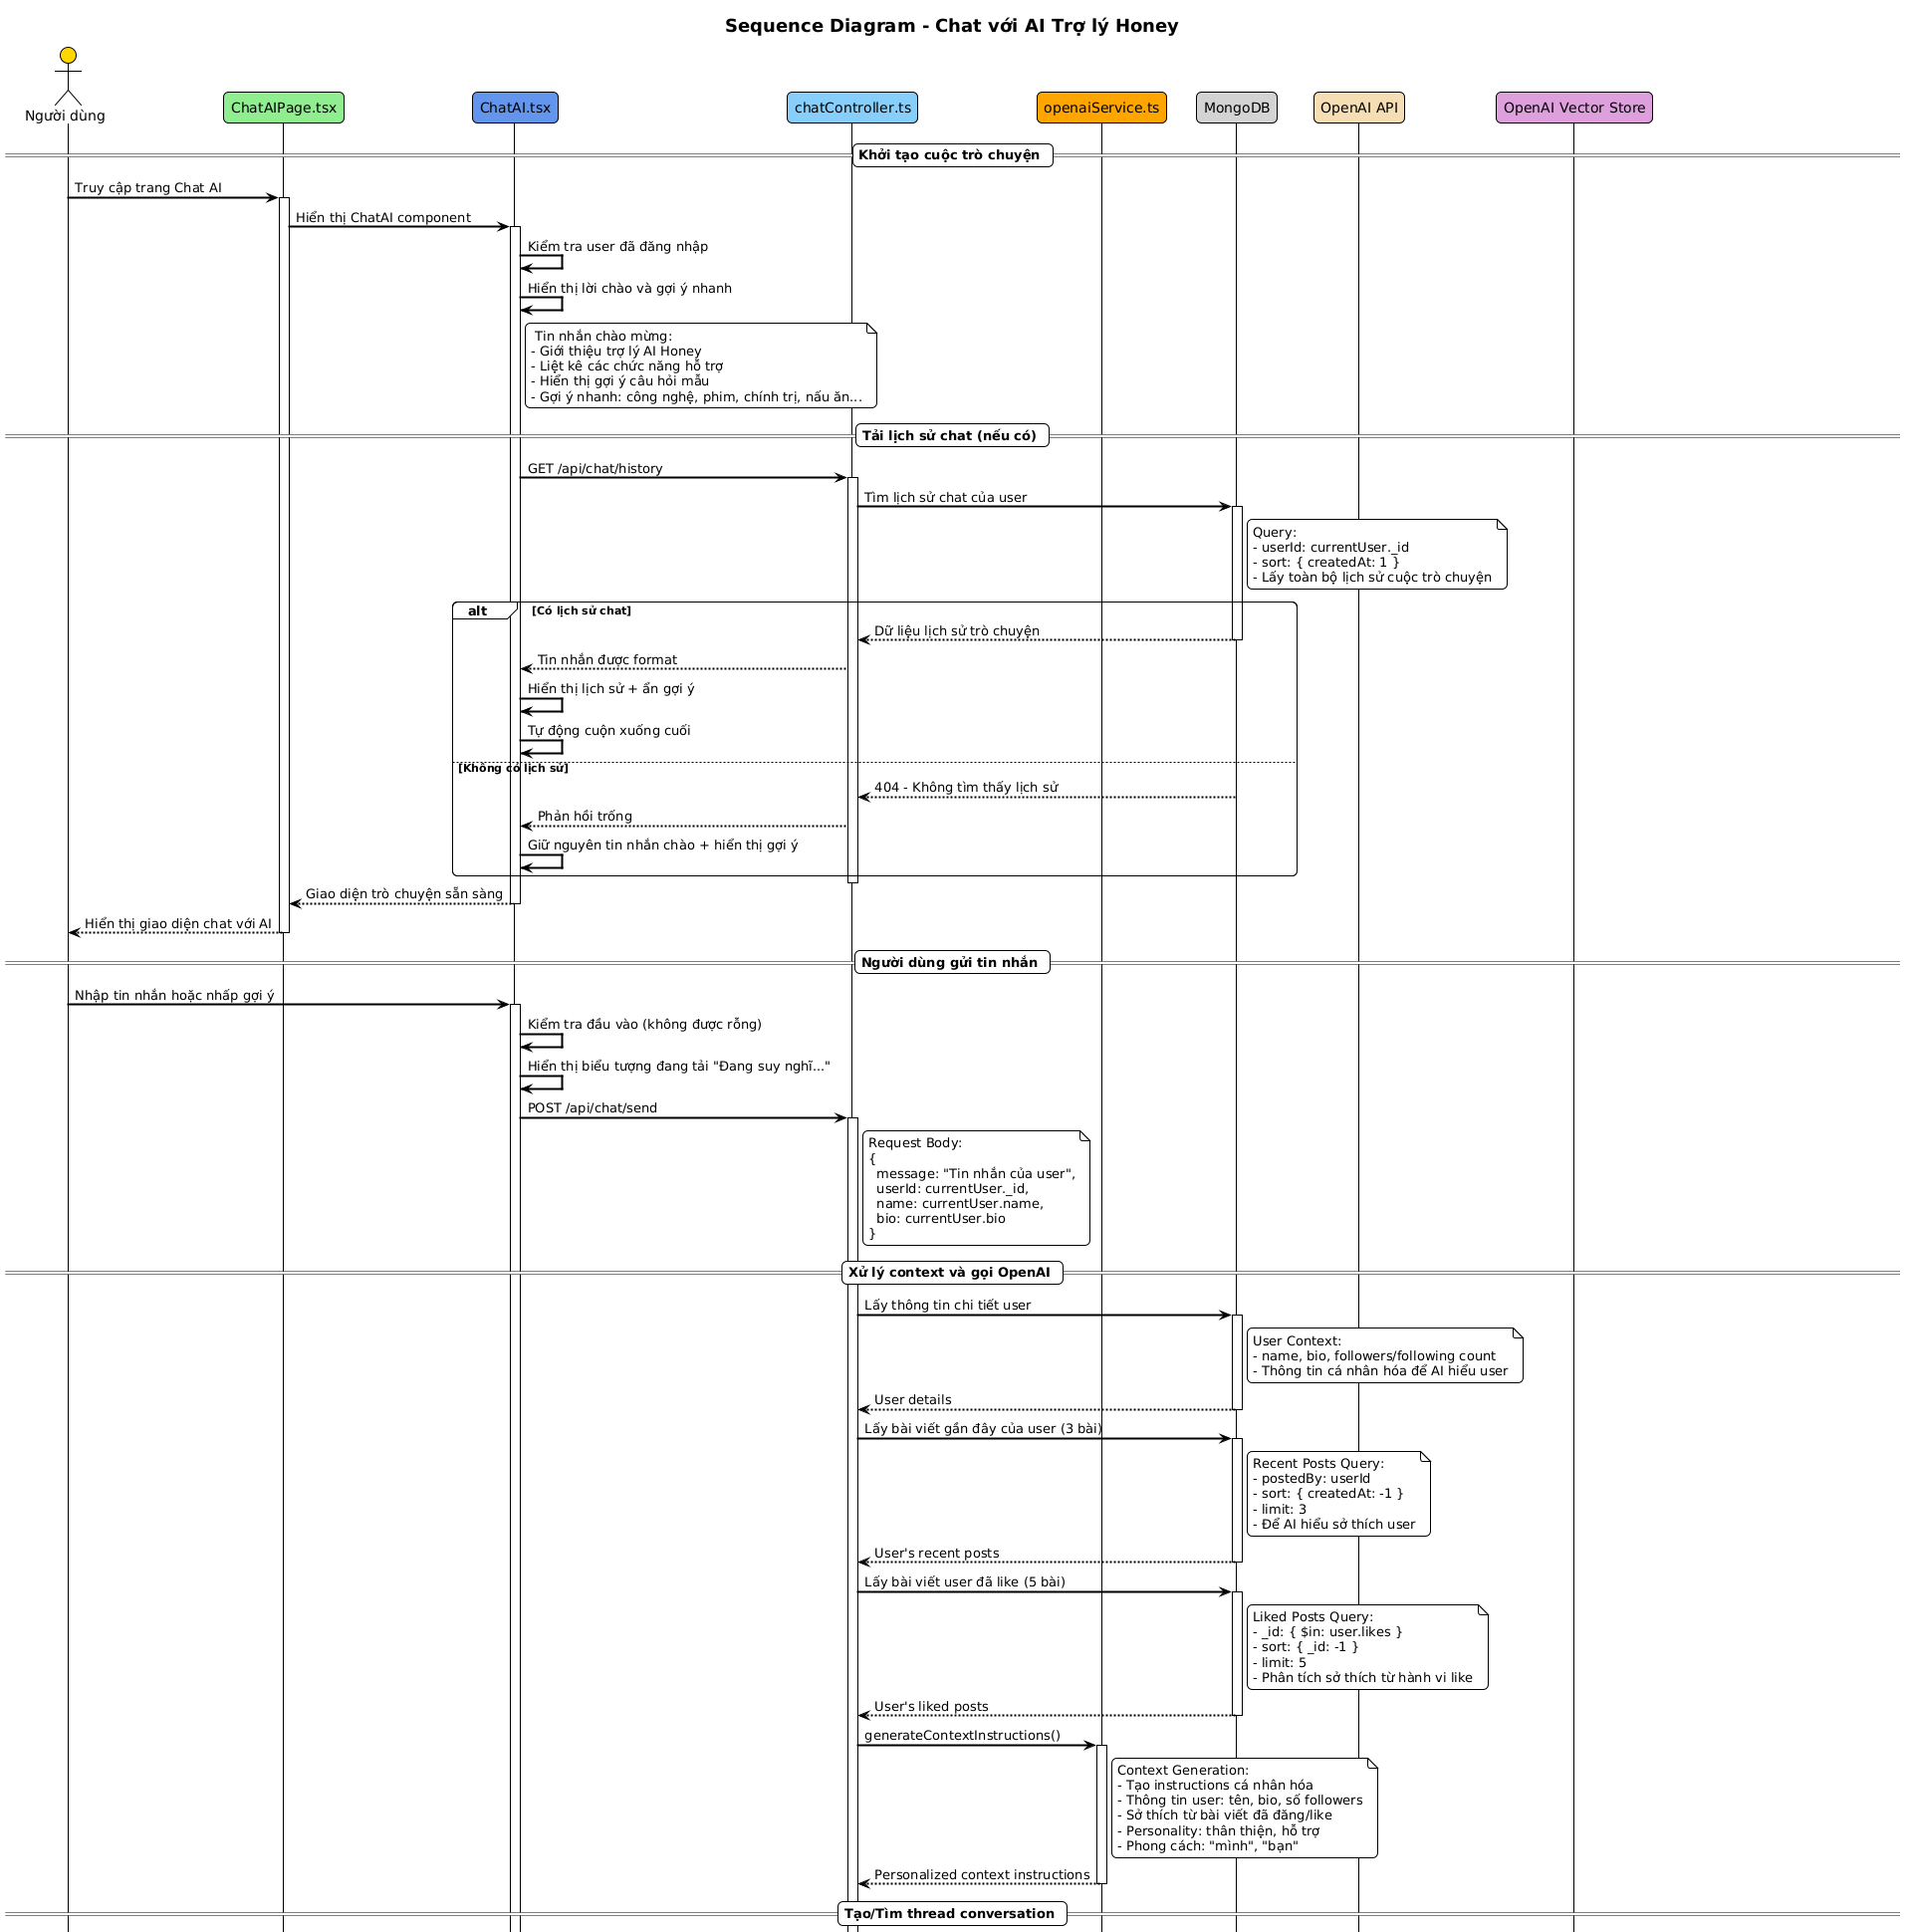
\includegraphics[width=1\textwidth]{image/sequence/chat-ai.png}
    \caption{Hình ảnh Chat AI}
    \label{fig:chat_ai}
\end{figure}


\begin{figure}[H]
    \centering
    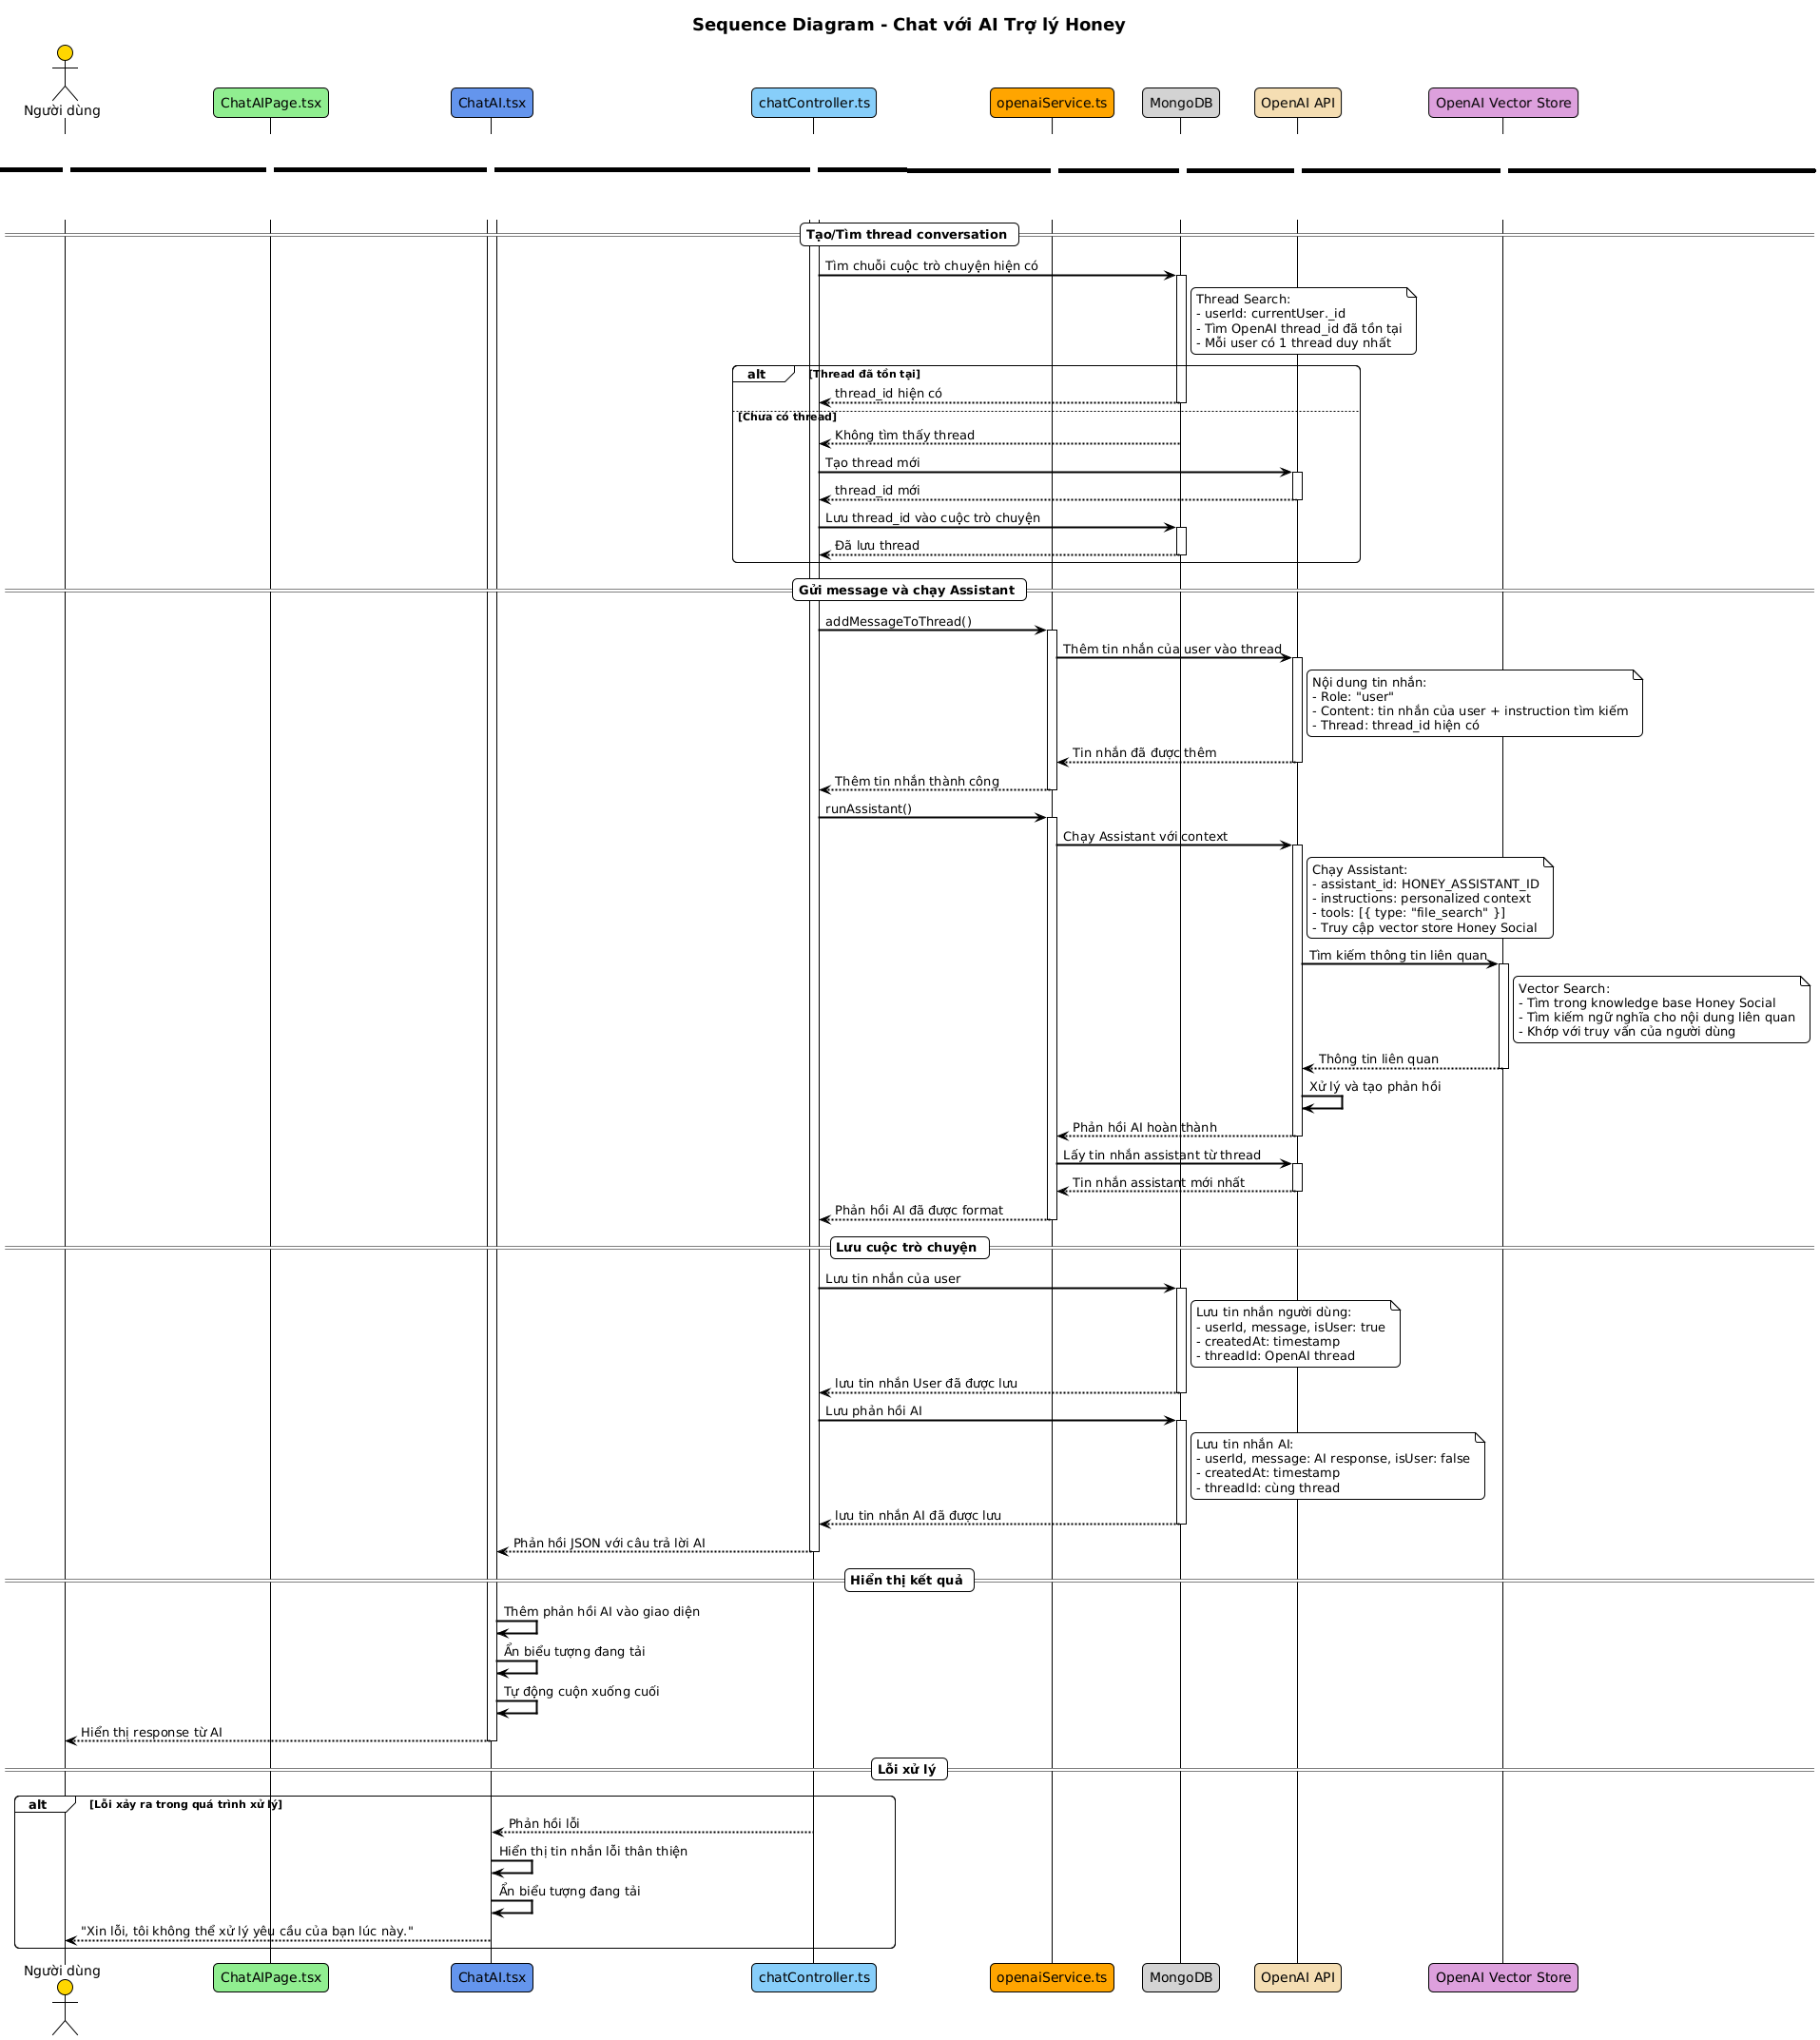
\includegraphics[width=1\textwidth]{image/sequence/chat-ai2.png}
    \caption{Hình ảnh Chat AI 2}
    \label{fig:chat_ai2}
\end{figure}


\begin{figure}[H]
    \centering
    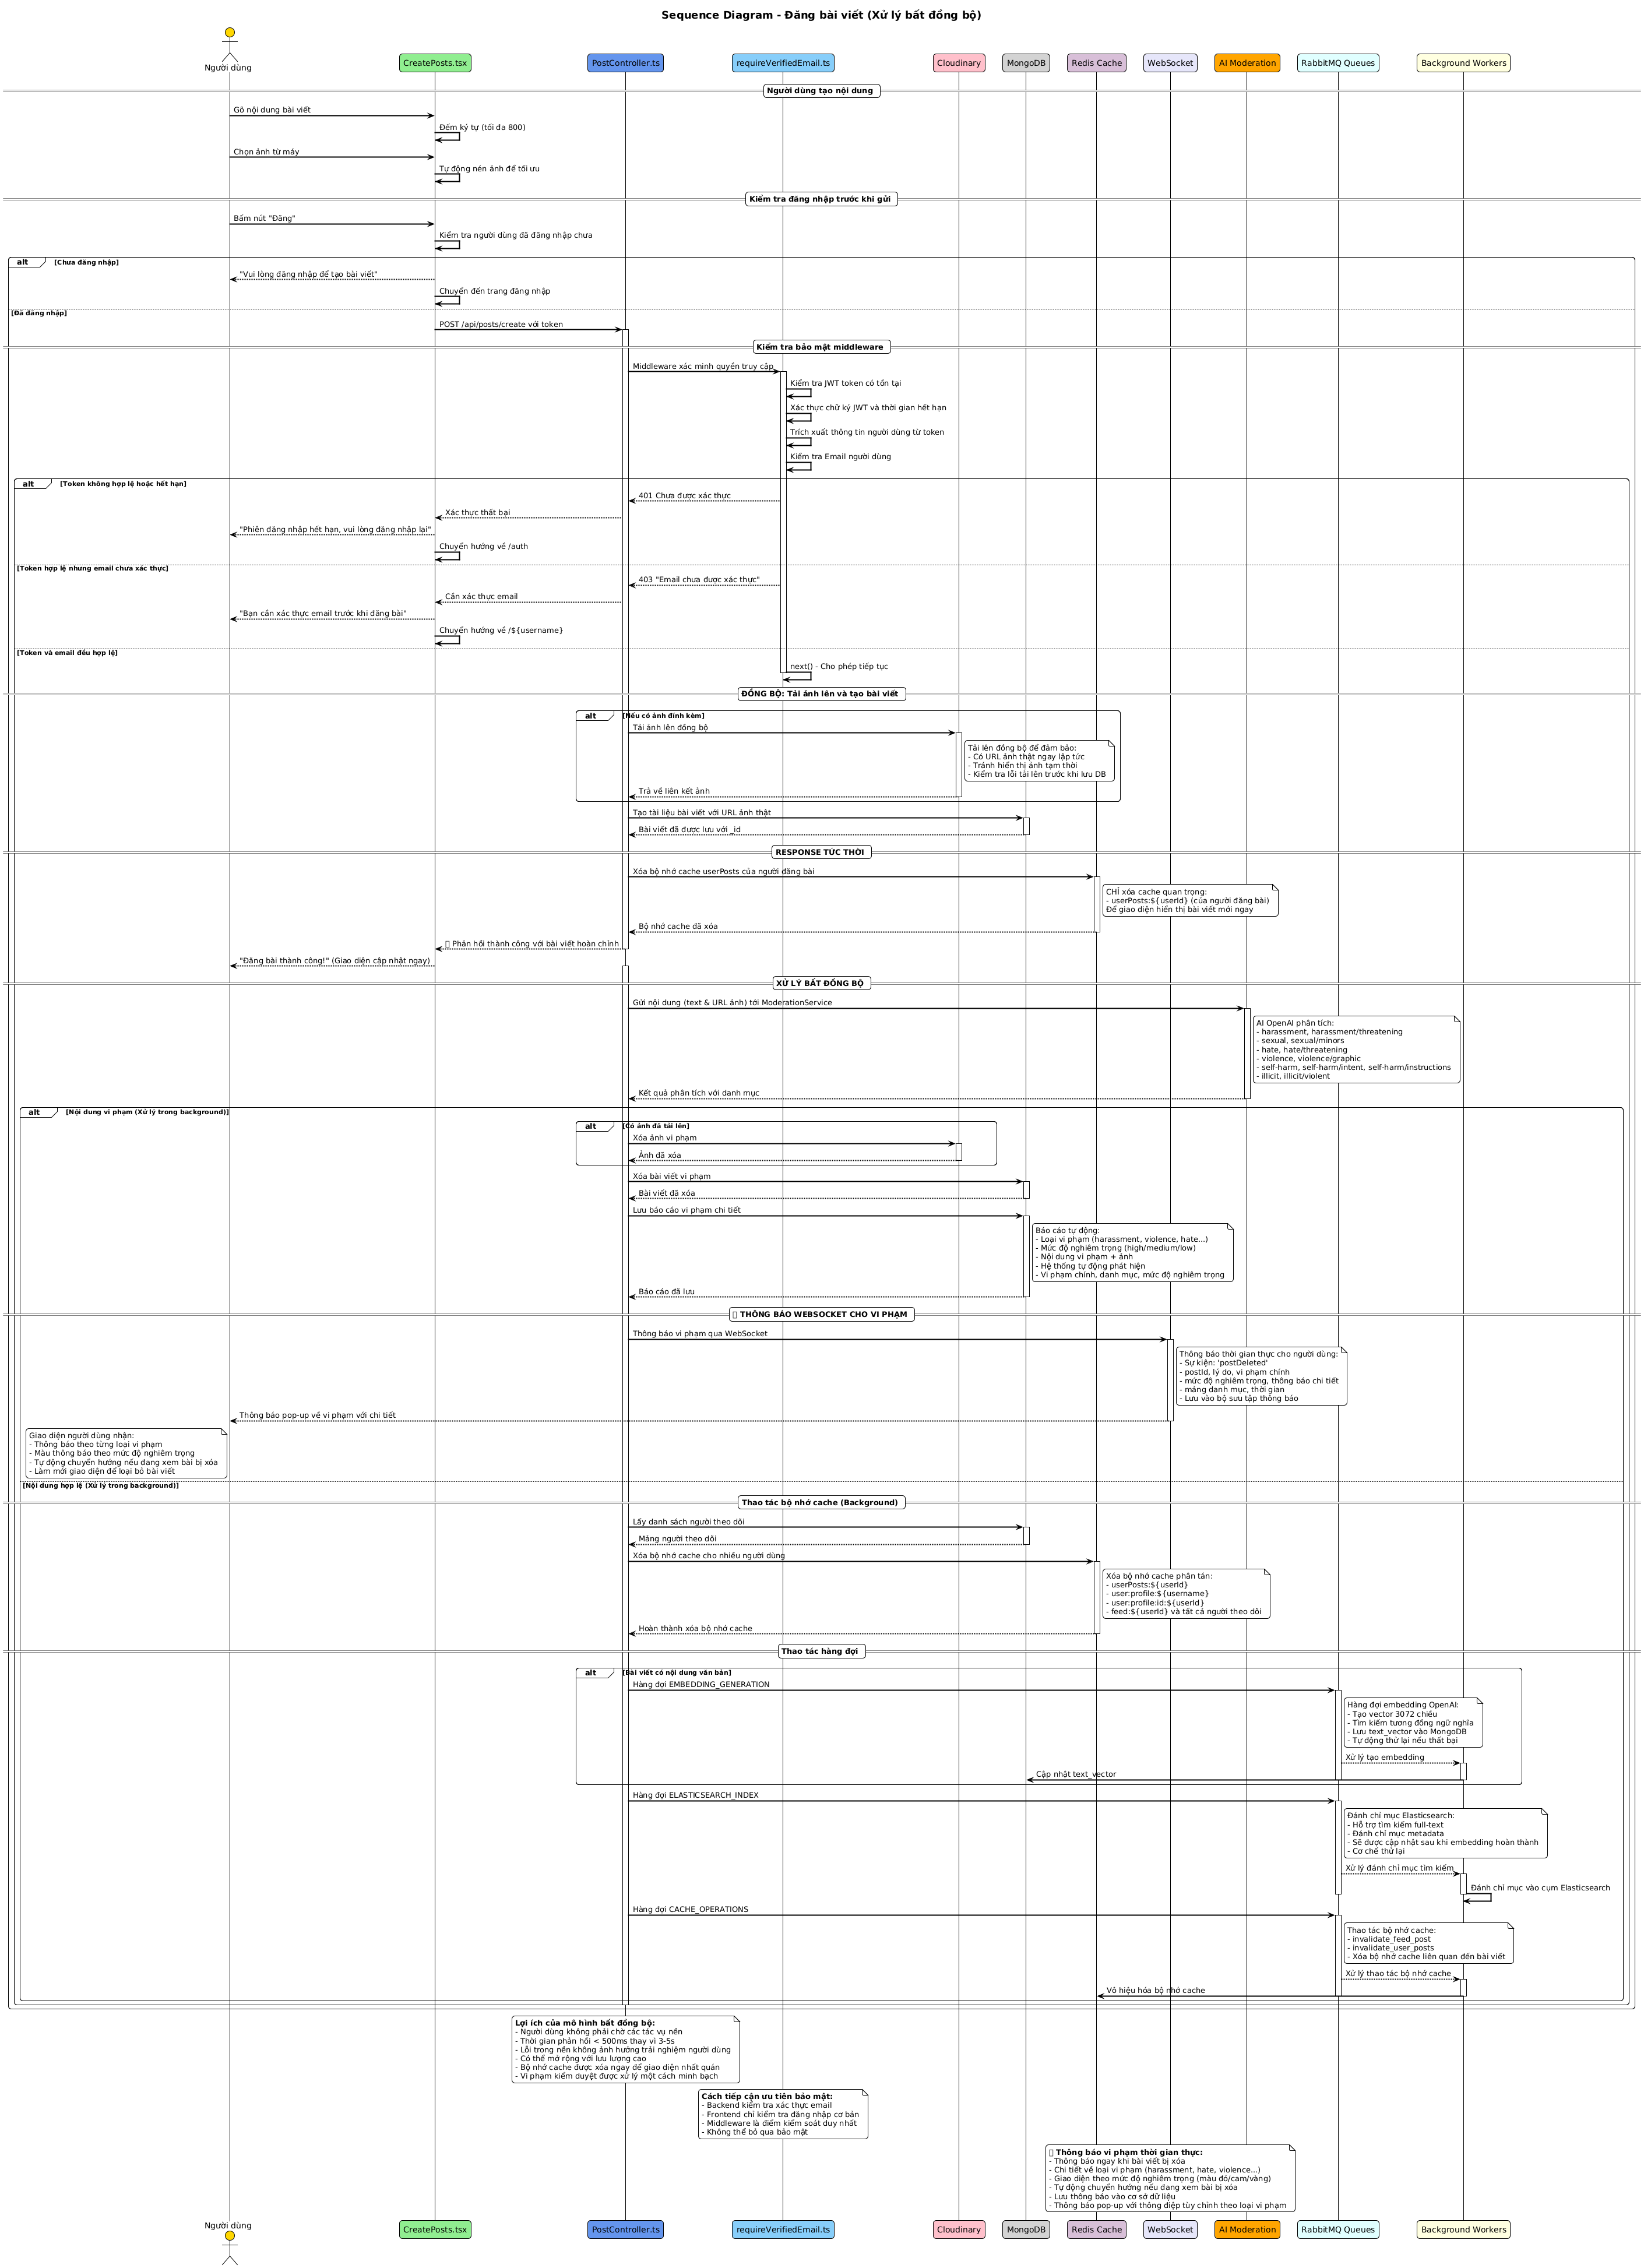
\includegraphics[width=1\textwidth]{image/sequence/dang-bai-viet.png}
    \caption{Hình ảnh Đăng bài viết}
    \label{fig:dang_bai_viet}
\end{figure}

\begin{figure}[H]
    \centering
    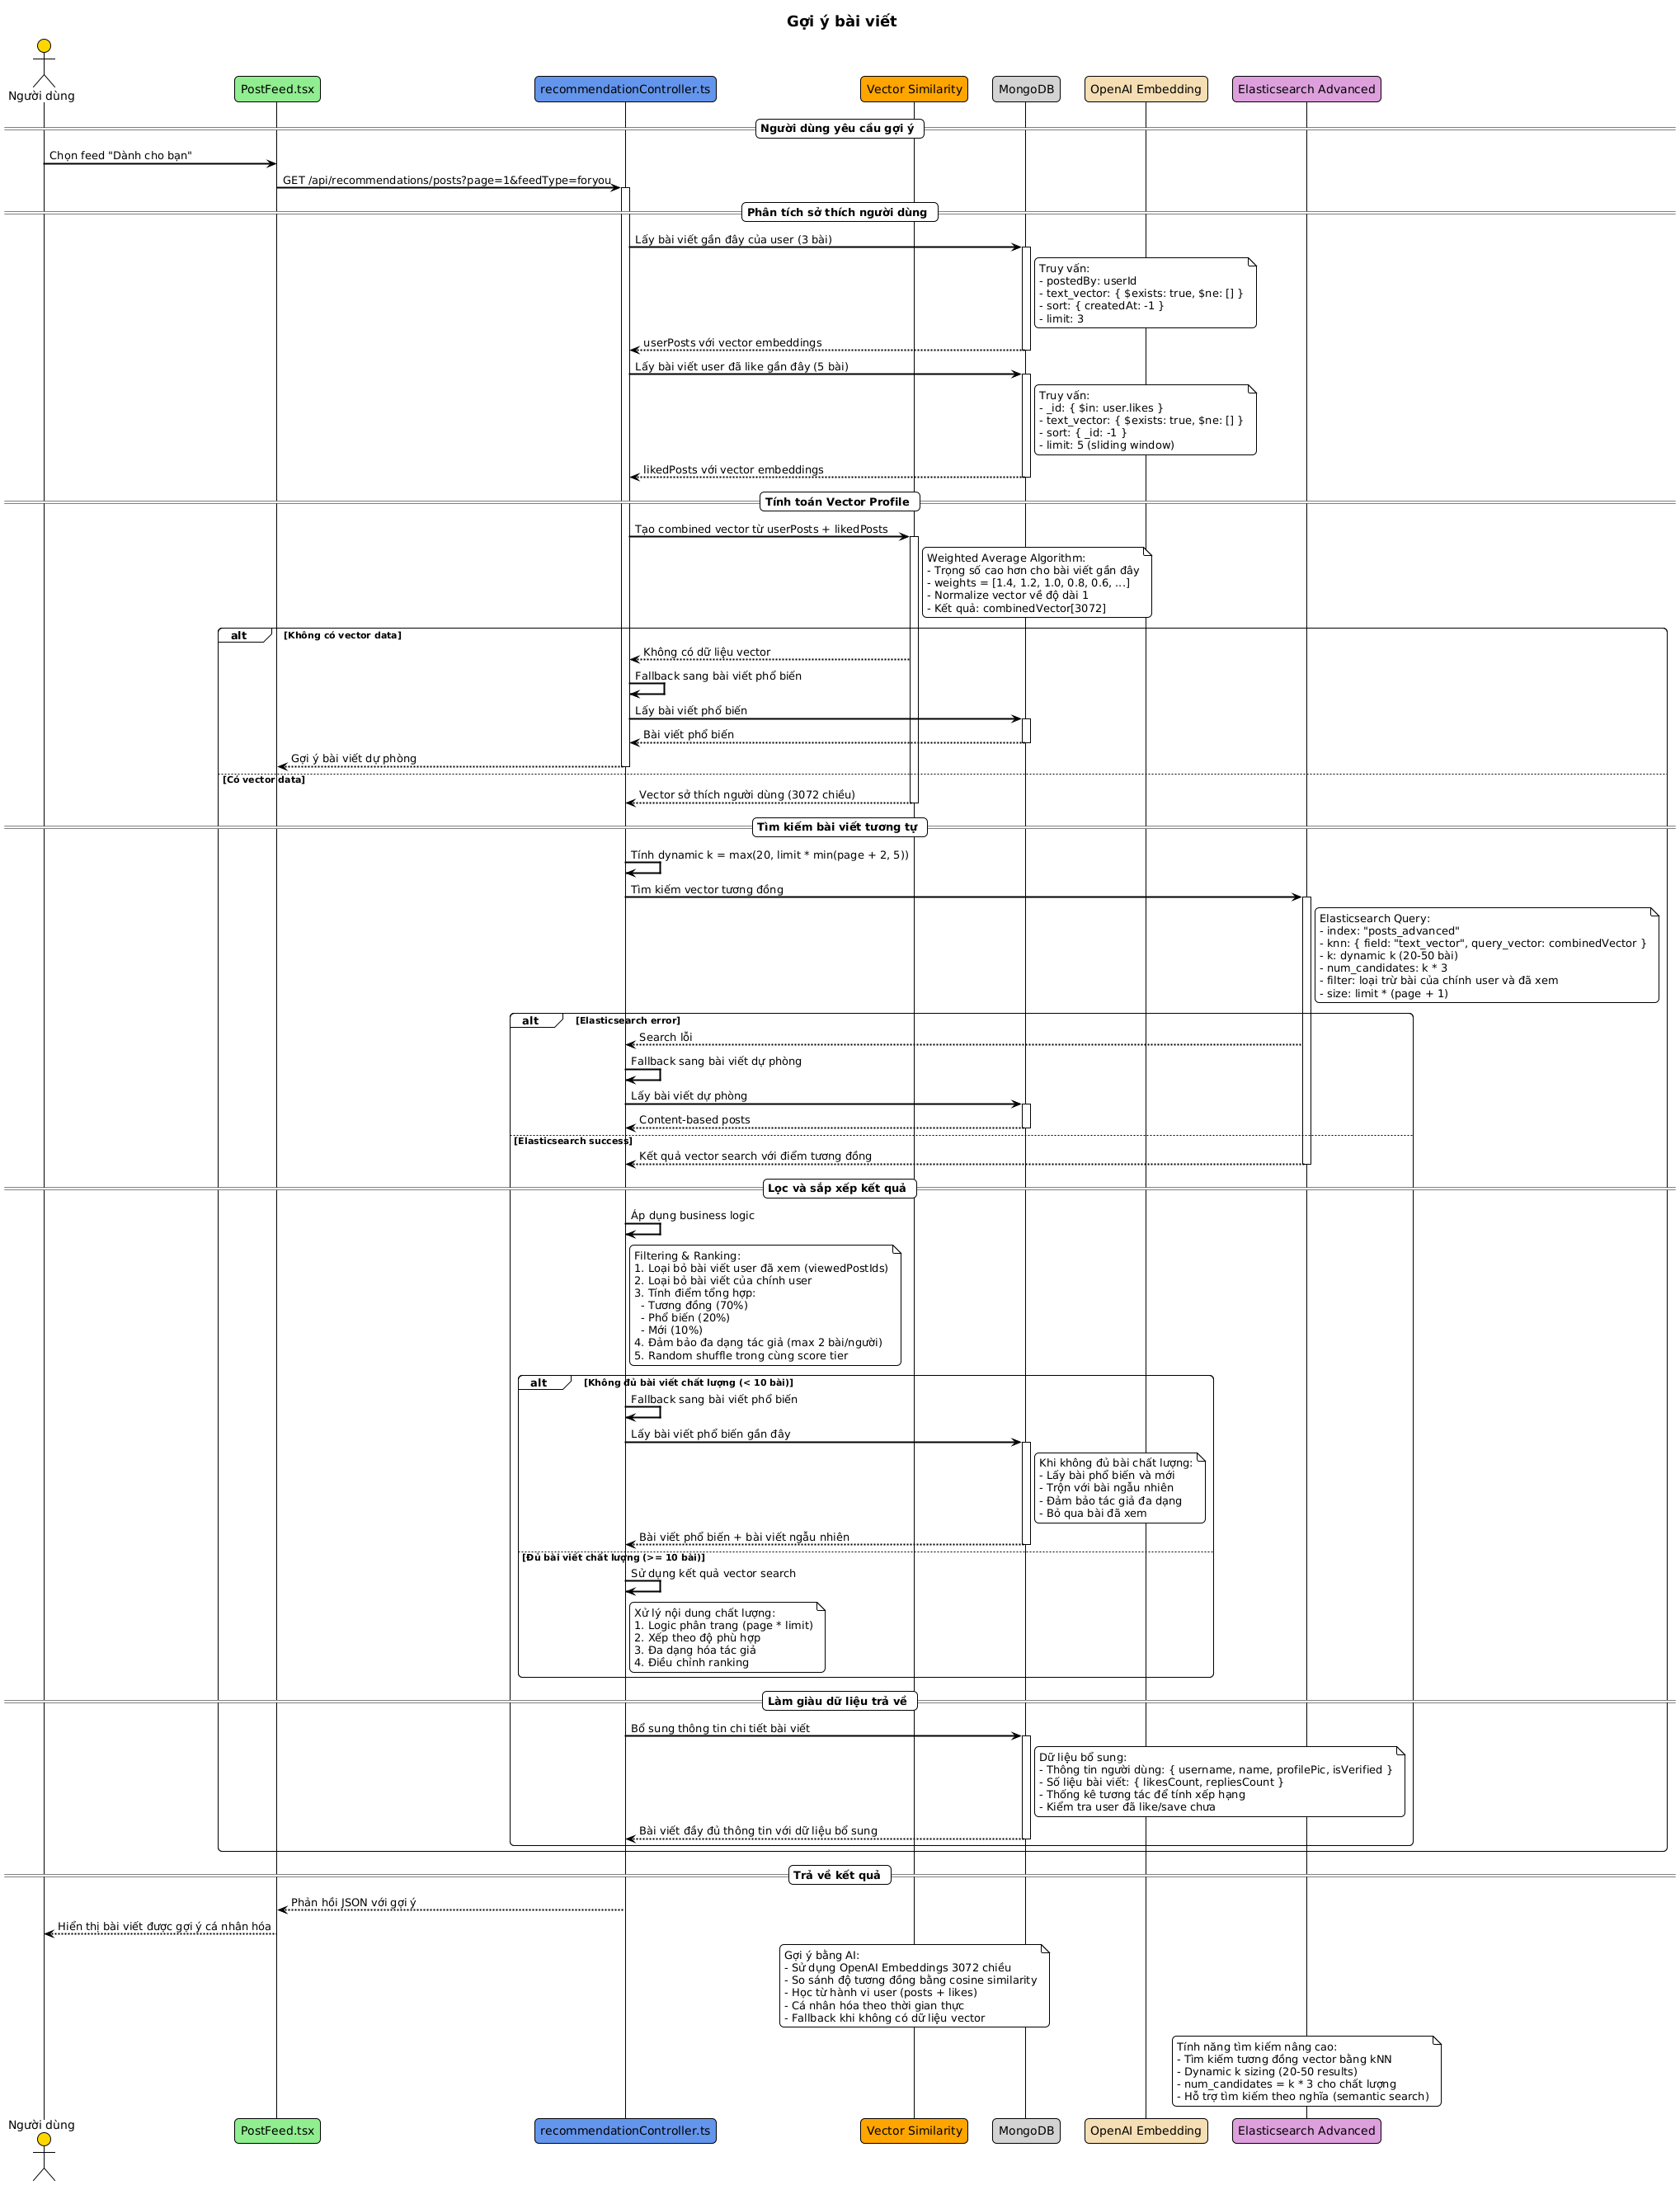
\includegraphics[width=1\textwidth]{image/sequence/goi-y-bai-viet.png}
    \caption{Hình ảnh Gợi ý bài viết}
    \label{fig:goi_y_bai_viet}
\end{figure}

\begin{figure}[H]
    \centering
    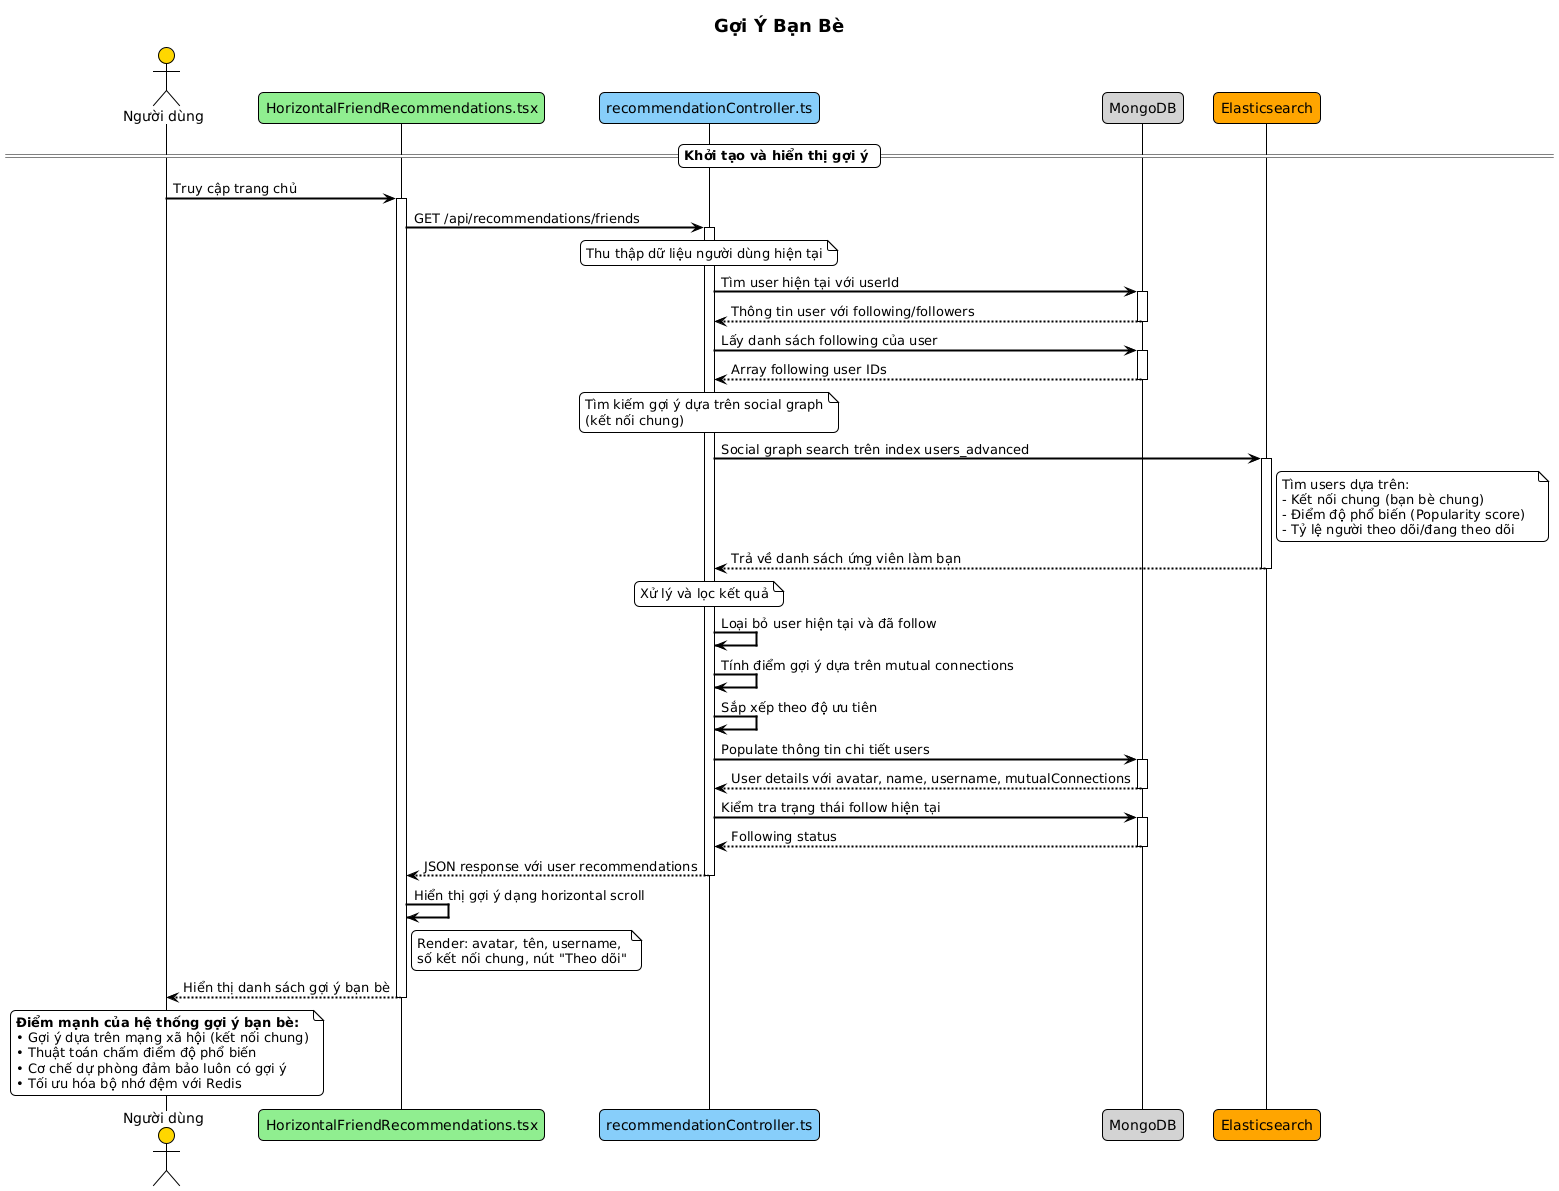
\includegraphics[width=1\textwidth]{image/sequence/goi-y-ban-be.png}
    \caption{Hình ảnh Gợi ý bạn bè}
    \label{fig:goi_y_ban_be}
\end{figure}


\begin{figure}[H]
    \centering
    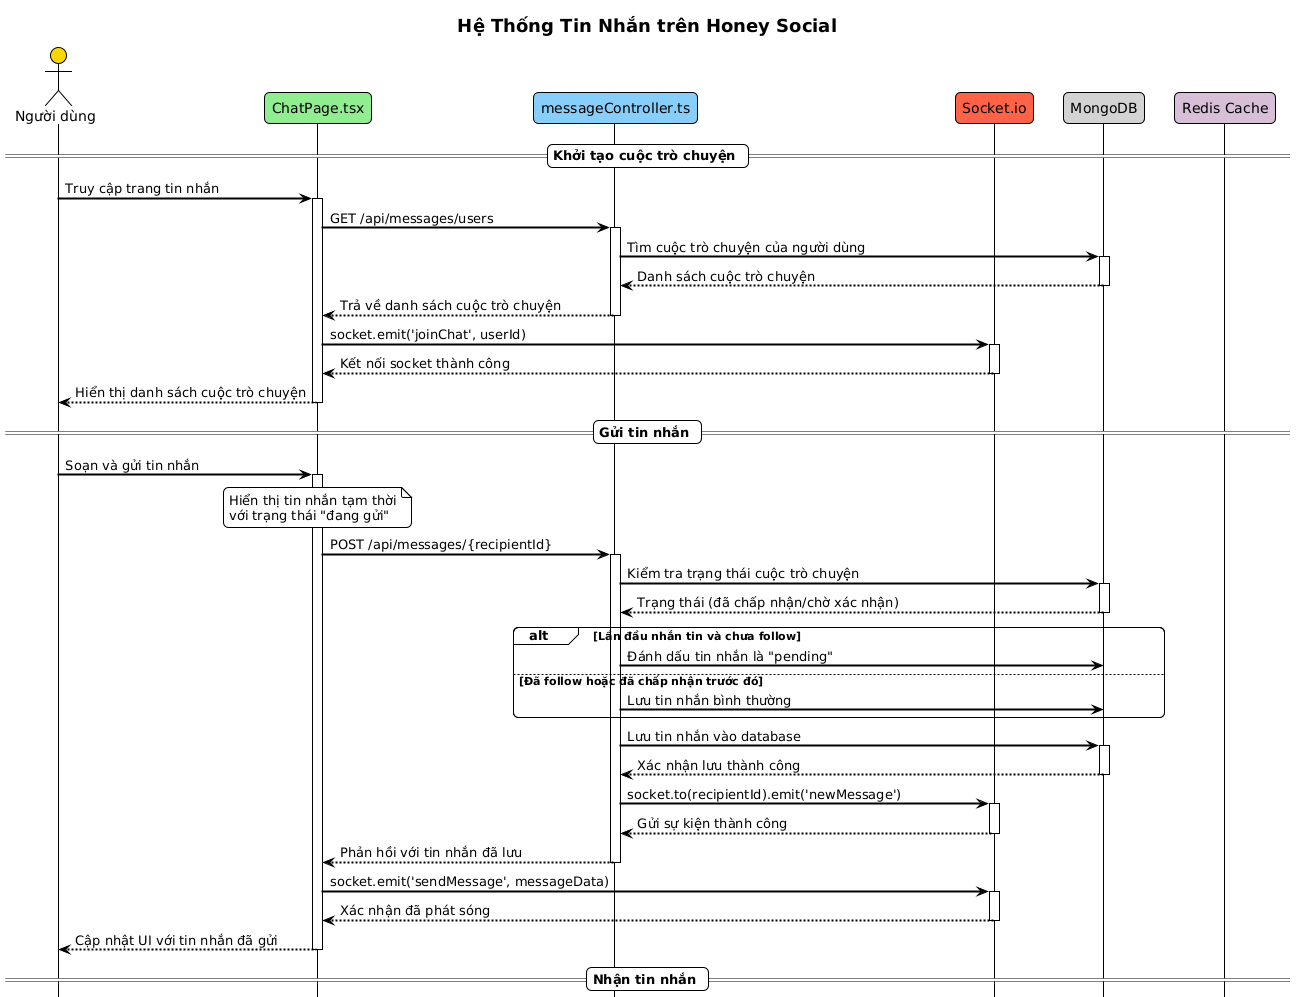
\includegraphics[width=1\textwidth]{image/sequence/message1.png}
    \caption{Hình ảnh Hệ thống tin nhắn trên Honey Social}
    \label{fig:message}
\end{figure}


\begin{figure}[H]
    \centering
    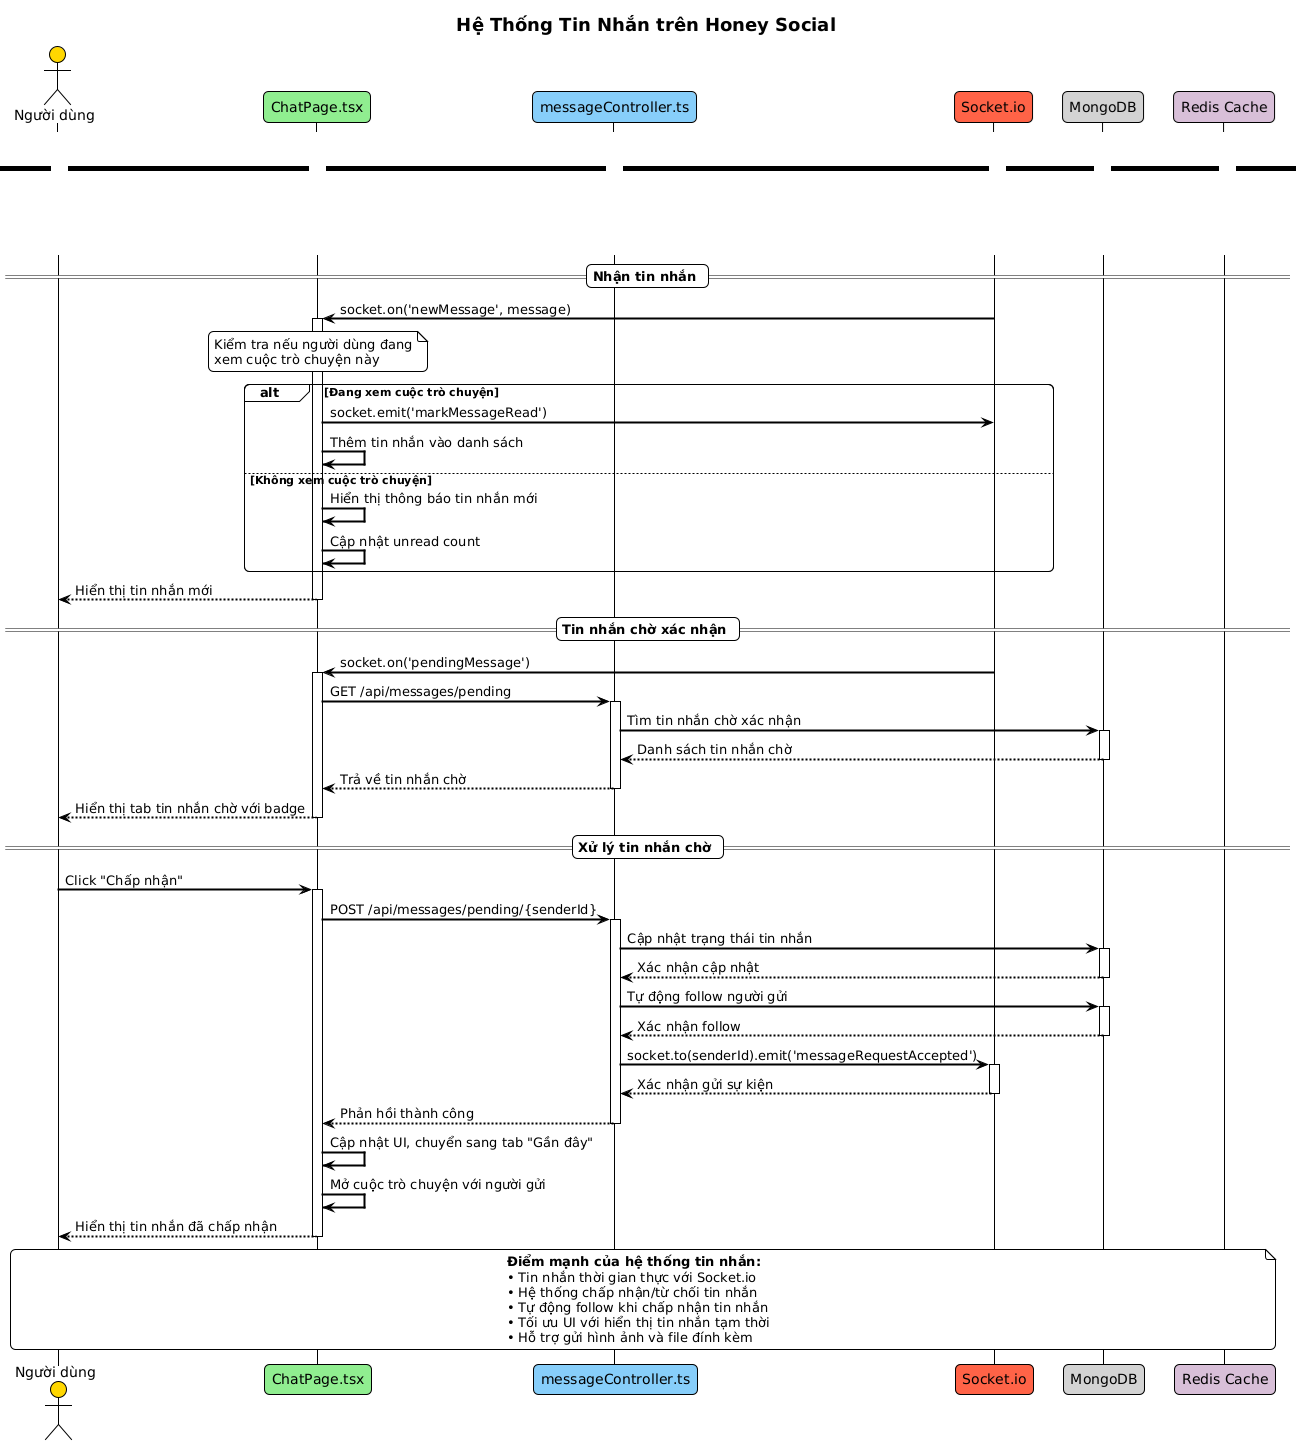
\includegraphics[width=1\textwidth]{image/sequence/message2.png}
    \caption{Hình ảnh Hệ thống tin nhắn trên Honey Social 2}
    \label{fig:message}
\end{figure}




\begin{figure}[H]
    \centering
    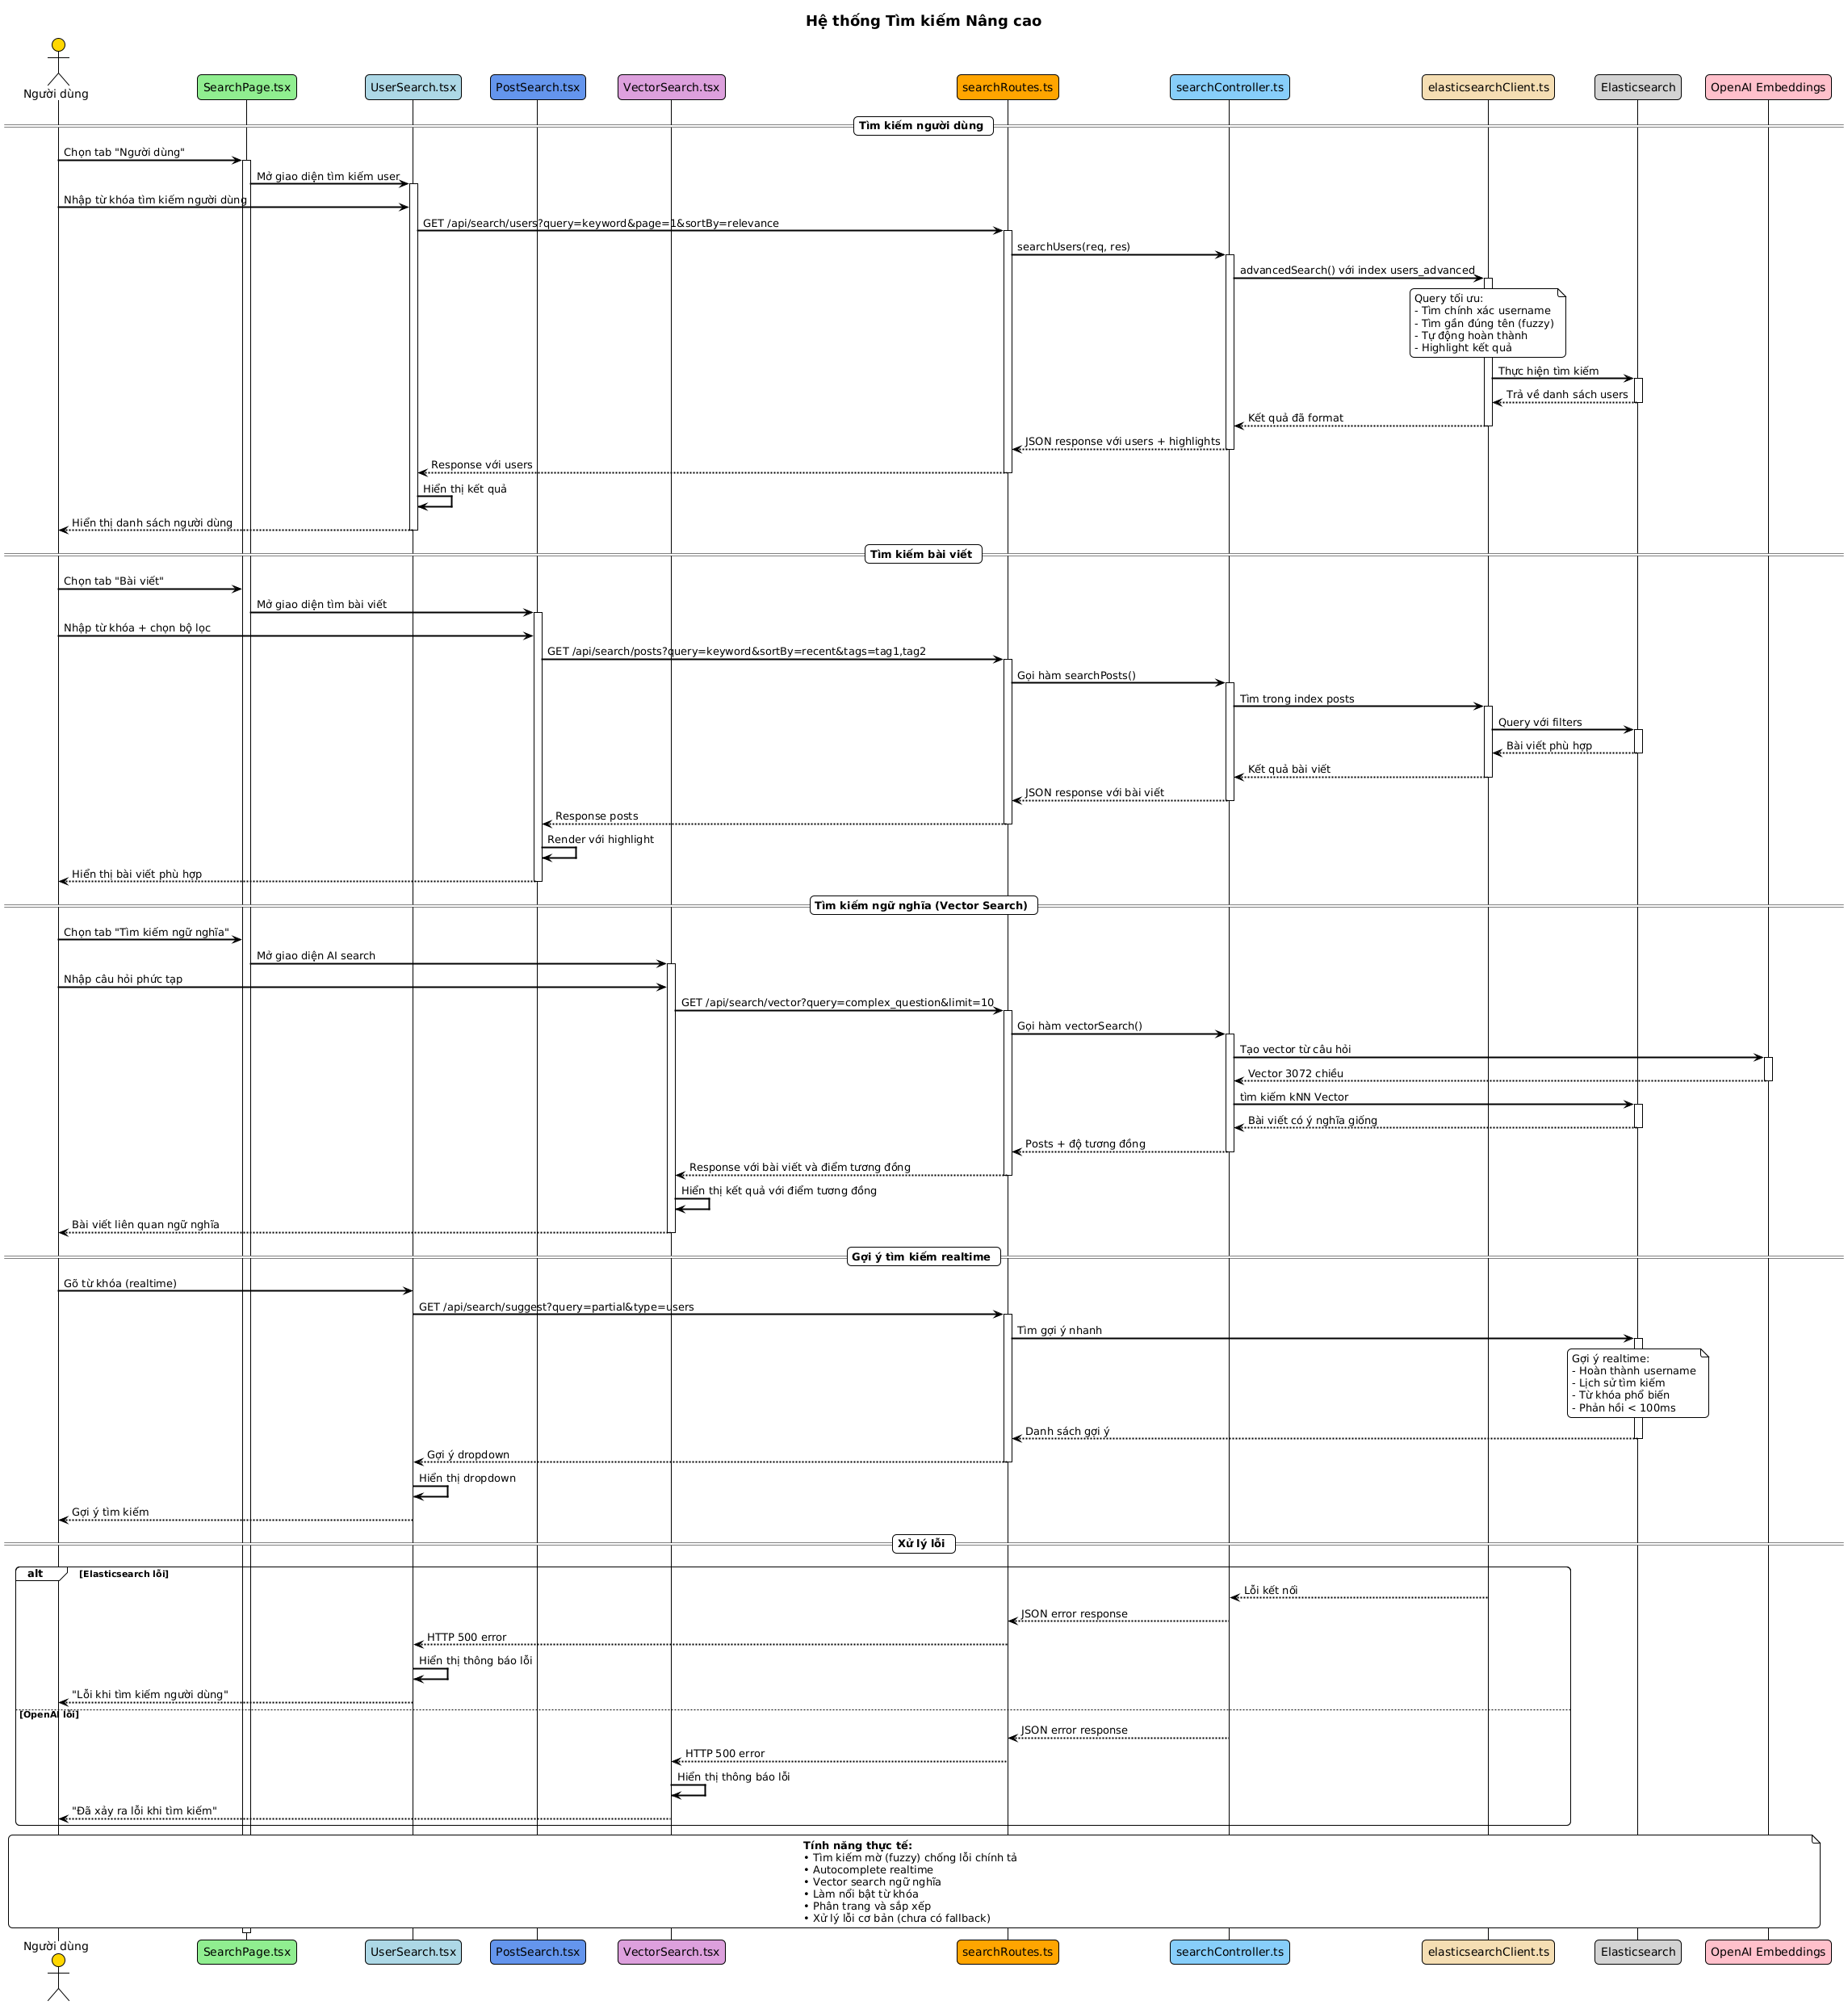
\includegraphics[width=1\textwidth]{image/sequence/tim-kiem-nang-cao.png}
    \caption{Hình ảnh Tìm kiếm nâng cao}
    \label{fig:tim_kiem_nang_cao}
\end{figure}
